
%: ----------------------- introduction file header -----------------------
\begin{savequote}[50mm]
At the end of a dream, if you know where I mean, when the mist just starts to clear.
% That's right here's where the talkin' ends.
\qauthor{Rainbow - Long Live Rock 'n' Roll}
\end{savequote}


\chapter{AdaptUIOnt: An Ontology for Dynamic User Interface Adaptation}
\label{cha:ontology_model}

\ifpdf
    \graphicspath{{3_ontology_model/figures/PNG/}{3_ontology_model/figures/PDF/}{3_ontology_model/figures/}}
\else
    \graphicspath{{3_ontology_model/figures/EPS/}{3_ontology_model/figures/}}
\fi

The existing literature approaches for user, context and device modelling
analysed in Chapter~\ref{cha:state_of_the_art} revealed several problems in
systems which aim the adaptation of user interfaces, applications or services.
To face these issues regarding a user interface adaptation the AdaptUI system
described in this dissertation proposes a platform supported by two main bases:
AdaptUIOnt, an ontology which describes the most significant concepts within a
user interface adaptation domain, and a set of rules, which main purpose is
to trigger different actions regarding the available knowledge of the current
domain represented through the ontology.

The following sections detail the concepts illustrated through Figure~\ref{fig:flow_diagram}.
This figure presents, on the one hand, several crucial concepts represented
through the AdaptUIOnt ontology. The ontology and all its characteristic are
detailed in Section~\ref{sec:adaptui_model}. On the other hand, the set of rules
which concern these concepts are also depicted. These rules are described in
Section~\ref{sec:adaptui_rules}. This first diagram is unfolded during this
chapter and finally reviewed in Section~\ref{sec:adaptui_conclusions} through
Figure~\ref{fig:flow_diagram_2} in order to update the illustration with all the
described model and the learned concepts.

\begin{figure}[H]
\centering
\includegraphics[width=0.75\textwidth]{flow_diagram.pdf}
\caption{Knowledge flow through the AdaptUI adaptation process. The circles
represent several main concepts presented in the AdaptUIOnt ontology. The arrows
describe the set of rules that affect the related concepts in the circles.}
\label{fig:flow_diagram}
\end{figure}

\section{The AdaptUIOnt Ontology}
\label{sec:adaptui_model}

As said before, the AdaptUI platform is supported by two pillars: an ontology
that models several significant concepts of the domain, and a set of rules
that trigger several modifications of these concepts. In this section the
AdaptUIOnt ontology, which represents the existing concepts in the user
interface adaptation domain, is presented.
  
The AdaptUIOnt ontology arises from the need of an adaptation model which gathers
knowledge of the \textit{user} capabilities, the \textit{context} that surrounds
the user, and the mobile \textit{device} the the user manipulates. The main goal
is to obtain a user interface adaptation personalized exclusively for the
characteristics of these three entities at the end of an adaptation process.

Through the following sections the AdaptUIOnt model is unfolded as follows: 
First, an introduction about the model is performed (see Section~\ref{sec:model_introduction}).
This introduction answers two design questions: \textit{how} the ontology has
been designed and \textit{why} several design decisions were made. The answers
bring several distinguishing aspects from the existing models found in the
literature (see Chapter~\ref{cha:state_of_the_art}). Next, in Section~\ref{sec:model_detail}
an answer to the question \textit{what} is given. The AdaptUIOnt ontology models
several primary and secondary groups of entities and knowledge. The primary
set of entities are grouped in the \textit{Entities Model}, explained in
Section~\ref{sec:entities_model}. The second group are contained in the
\textit{Dynamic Entities}, explained in Section~\ref{sec:dynamic_model}. Besides,
AdaptUIOnt describes several concepts and supports a set of rules which trigger
different actions (see Section~\ref{sec:adaptui_rules}).


\subsection{Introducing AdaptUIOnt: The \textit{Hows} and the \textit{Whys}}
\label{sec:model_introduction}

The literature analysis made in Chapter~\ref{cha:state_of_the_art} exposes
several possibilities regarding the problem of choosing the best technique
to model a user interface adaptation process and all the required knowledge
around it. As it will be explained later in the conclusions of this chapter, we
found that using ontologies would bring several benefits to our proposal. In 
this section we explain \textit{how} and \textit{why} the AdaptUIOnt ontology 
has been designed.

Many ontology based solutions take users as entities described by their physiological
capabilities~\citep{gregor_designing_2002}~\citep{razmerita_ontology_based_2003}
\citep{pereira_triple_2005}~\citep{persad_characterising_2007}~\citep{persad_cognitive_2007}
and~\citep{skillen2012ontological}. Moreover, facing adaptation or personalization
problems these solutions aim to cover not only capabilities but also disabilities.
When AdaptUIOnt was conceived, we found that modelling physiological abilities
was not practical. Although many users may have similar preferences and capabilities,
their tastes may differ. Besides, their reactions facing several problems may not
be the same. In addition, we realised how difficult it is to model each user
physiological characteristics without an expert's support. As scientists in the
computing domain we lack of this kind of physiological knowledge about individuals.
Thus, we believe we cannot face modelling user capabilities and also contemplating
and analysing their behaviour and responses.

Nevertheless,~\citet{casas_user_2008} described a taxonomy where user disabilities
are not explicitly contemplated. Instead of that, user preferences are classified
under several concepts, as is shown in Figure~\ref{fig:casas}. Through the taxonomy
represented by this figure it is shown how the authors avoid the modelling of
physiological capabilities of the user, centring the model in several preferences.
More information about the considerations of Casas et al. are given in
Section~\ref{sec:casas}.


\begin{figure}
\centering
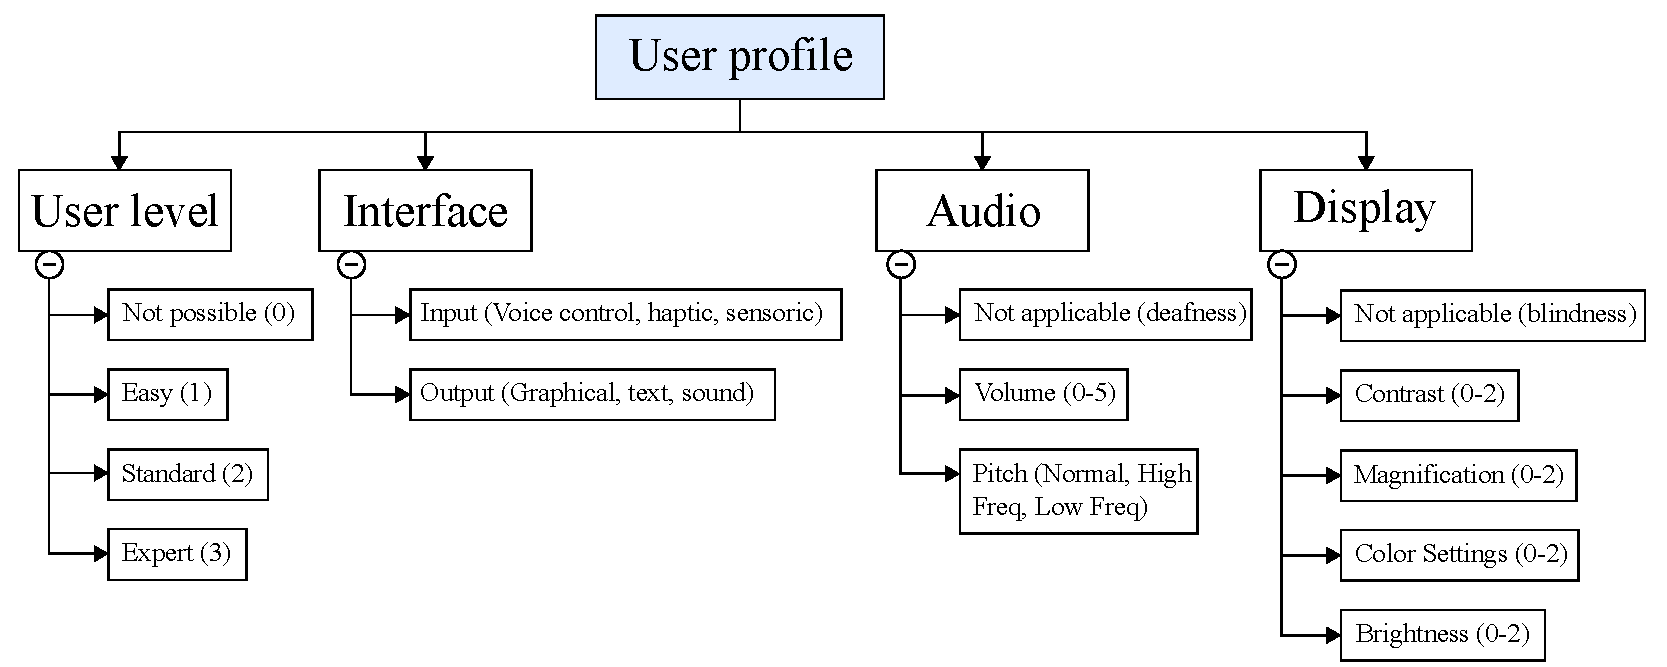
\includegraphics[width=1.0\textwidth]{../figures/PDF/casas.pdf}
\caption{User profile taxonomy by~\citet{casas_user_2008}.}
\label{fig:casas}
\end{figure}

AdaptUIOnt is built under this idea, extending it and avoiding the modelling of
any explicit physiological characteristics. As it will be depicted in this chapter
several concepts changed in our proposal. Besides, several remarkable ontologies
from other authors are also used to enrich the AdaptUIOnt knowledge. For example,
the \ac{foaf} ontology~\citep{foaf} has been linked to complete the information 
of the user. The same happens with the \ac{gumo}~\citep{heckmann_gumogeneral_2005}, 
which also models information about the user. Although not all classes are 
included, several have been imported in the final version of the AdaptUIOnt 
model, as they might represent significant concepts for other developers. 
For example, in the \ac{gumo} ontology there is a class which models the user 
emotional state (\textit{Basic User Dimensions} $\rightarrow$ 
\textit{Emotional State}) through five basic emotions. In  the current AdaptUIOnt 
version these emotions are not considered for the adaptations. However, we believe
that other developers may consider that being under an \textit{anxiety} condition
might change or modify the result or the adaptation process. Every ontology that
has been used to complete the AdaptUIOnt ontology is shown in Table~\ref{tbl:used_ontologies}.

\begin{table}[H]
  \caption{Imported ontologies to complete several concepts of the AdaptUIOnt
  ontology: \ac{gumo}, \ac{foaf} and \ac{cobra}.}
 \label{tbl:used_ontologies}
\footnotesize
\centering
 \begin{tabular}{l l l l}
  \hline 
  \textbf{Ontology} 		& \textbf{Class}		& \textbf{Description}		& \textbf{Imported subclasses}		\\
  \hline
  \ac{gumo}~\citep{heckmann_gumogeneral_2005}& \textit{Basic User Dimensions}& It originally models 	& \textit{Ability And Proficiency},\\
				& 				& different aspects of 		& \textit{Characteristics},		\\
				& 				& the user, as certain 		& \textit{Contact Information},		\\
				&				& abilities, emotional 		& \textit{Demographics},		\\
				&				& status, and so on.		& \textit{Motion}, \textit{Role},	\\
  				& 				&  				& \textit{Emotional State},		\\
  				& 				&  				& \textit{Personality}, \textit{Mental}	\\
  				& 				&  				& \textit{State}, \textit{Physiological}\\
  				& 				&  				& \textit{State}			\\
  				& \textit{Context Information}	& It represents several		& \textit{Location} and \textit{Physical}\\
  				&				& concepts related to 		& \textit{Environment} and \textit{Social}\\
  				&				& the environment.		& \textit{Environment}.			\\
  \ac{foaf}~\citep{foaf}	& \textit{Document}		&  	 			& \textit{Image} and 			\\  
				& 				&				& \textit{PersonalProfileDocument}.	\\
				& \textit{SocialInstitution}	& 				& 					\\
				& \textit{OnlineAccount}	& 				& \textit{Online Chat Account},		\\
				& 				&				& \textit{Online E-commerce} 		\\
				& 				&				& \textit{Account} and \textit{Online} 	\\
				& 				&				& \textit{Gaming Account}.		\\
  \ac{cobra}~\citep{cobra}	& \textit{DeviceMemory}		& 				& 					\\
				& \textit{DisplayScreen}	& 				& 					\\
				& \textit{DisplayScreenResolution}& 				& 					\\
				& \textit{MemoryUsageType}	& 				& 					\\
  \hline
  
\end{tabular}
\end{table}


Other works have also been taken into account for the user model. For example
~\citet{gregor_designing_2002} consider that users (in this case, the elderly)
evolve and their capabilities might change not just because of their experience
but because of the context influence. For Gregor et al. elderly's capabilities
decrease due to their ageing. In this dissertation, this evolution of the user
capabilities is considered to be based on the context conditions and experience.
This is explained in Section~\ref{sec:adaptation_polisher}, in which a concrete
module of the AdaptUI architecture is introduced.

Through the AdaptUIOnt's user model we also aim to allow users to configure
the adaptation process through the cited perspective, which is, without any required
physiological knowledge. During this configuration the user interacts with a
module called Capabilities Collector indicating several interaction requirements.
This module translates the user indications into a capabilities module. The
Capabilities Collector and all its features are detailed in
Section~\ref{sec:capabilities_collector}.

Regarding the context, several considerations were also discussed during the design
process. Context is mainly defined by its physiological conditions. Besides,
the \ac{gumo}~\citep{heckmann_gumogeneral_2005} ontology has been used to enrich the
model. The context model is extended in two different ways: on the one hand,
there is the sensors information and the combination of their measures (environment
data); on the other hand, a high-level information category built from the
combination of context and external pieces of information.

Devices are also modelled using different \ac{cobra}~\citep{cobra} classes. These
classes represent static and dynamic concepts of the device. Device's screen
resolution (\textit{DisplayScreenResolution}) is one of the static features of a
mobile device. On the contrary, the battery of the device changes with the use.
This is represented through the \textit{Battery} class, and is also used by
AdaptUIOnt to represent this concept. AdaptUIOnt remarks the dynamic characteristics
of these devices, which are usually not modelled and are vital for the result of
any kind of adaptation. Thus, several classes representing dynamic characteristics
of mobile devices are added.



\subsection{Designing the AdaptUIOnt Ontology}
\label{sec:model_detail}

The AdaptUIOnt ontology has been designed with two main considerations in mind.
First, taking into account that useful and practical (and non physiological)
capabilities of the user, context and device need to be represented in the model.
This is carried out by reviewing the literature models and making several
adaptations, modifications and contributions. For example, regarding the user
model, we use \ac{foaf}~\citep{foaf} and \ac{gumo}~\citep{heckmann_gumogeneral_2005} to
model the user most personal characteristics. Nevertheless, the user model is
not based on these ontologies. It is built under several assumptions made by
\citet{casas_user_2008} in their user profile taxonomy, with several modifications.
Regarding the three entities, the ontology understands each one as a set of
characteristics that define them. Thus, there is, for example, a \textit{User}
class with a relationship \textit{definedBy} which relates the concept of a user
with the characteristics that define him/her (the \textit{UserCharacteristics}
class). The same conceptualization is shared by the other two entities (see
Figure~\ref{fig:entities_characteristics}). This part of the ontology has been
called \textit{Entities Model}, and it is detailed in Section~\ref{sec:entities_model}.



\begin{figure}
\centering
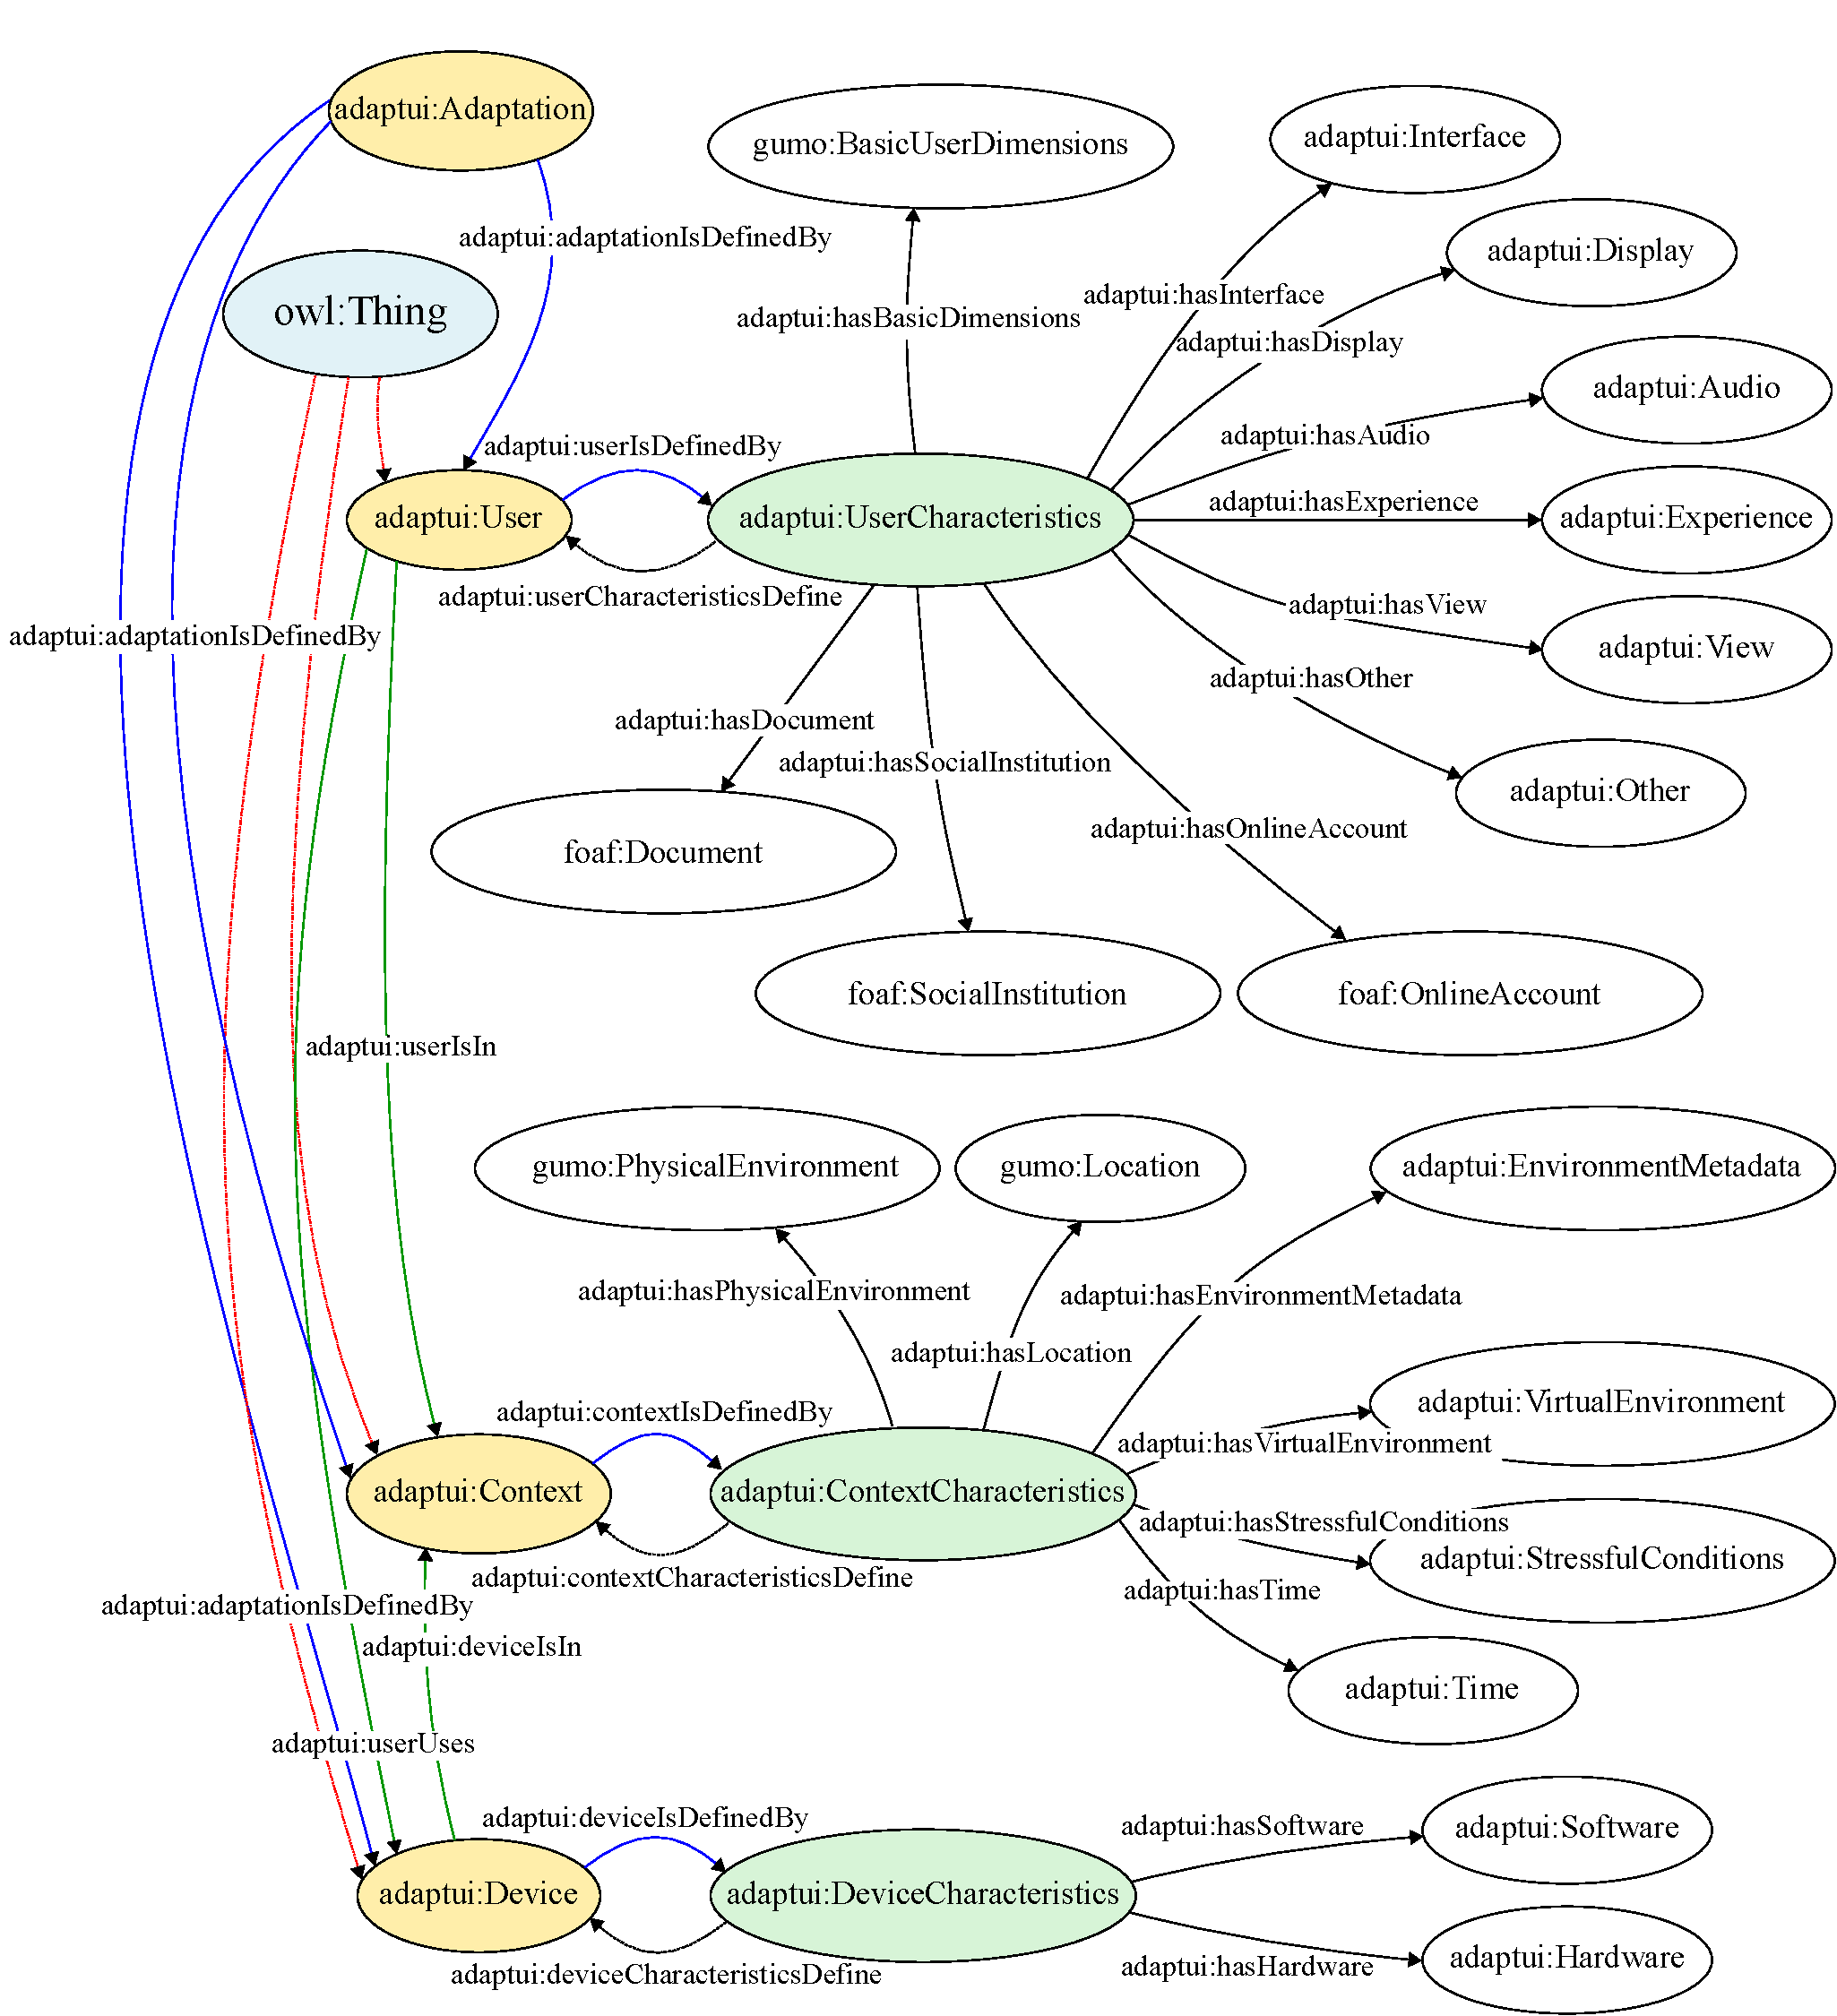
\includegraphics[width=0.90\textwidth]{../figures/PDF/entities_characteristics}
\caption{\textit{User},
\textit{Context} and \textit{Device} classes (in yellow) and their main object
relationships. As is shown, these classes are defined by their corresponding
characteristics class (in green).}
\label{fig:entities_characteristics}
\end{figure}


Second, and based on the conclusions made by~\citet{gregor_designing_2002},
the proposed ontology aims to be aware of the possible dynamic variations of the
environment, which may affect to the three entities. Therefore, we have implemented
several auxiliary classes to collect all the temporary knowledge within the
environment. These classes, shown in Figure~\ref{fig:auxiliary_classes}, are
linked to the main classes and complete them through several triggered rules
(see Section~\ref{sec:adaptui_rules}). This part of the dynamic knowledge
representation of the AdaptUIOnt ontology has been called \textit{Dynamic Model},
and it is explained in Section~\ref{sec:dynamic_model}.


\begin{figure}
\centering
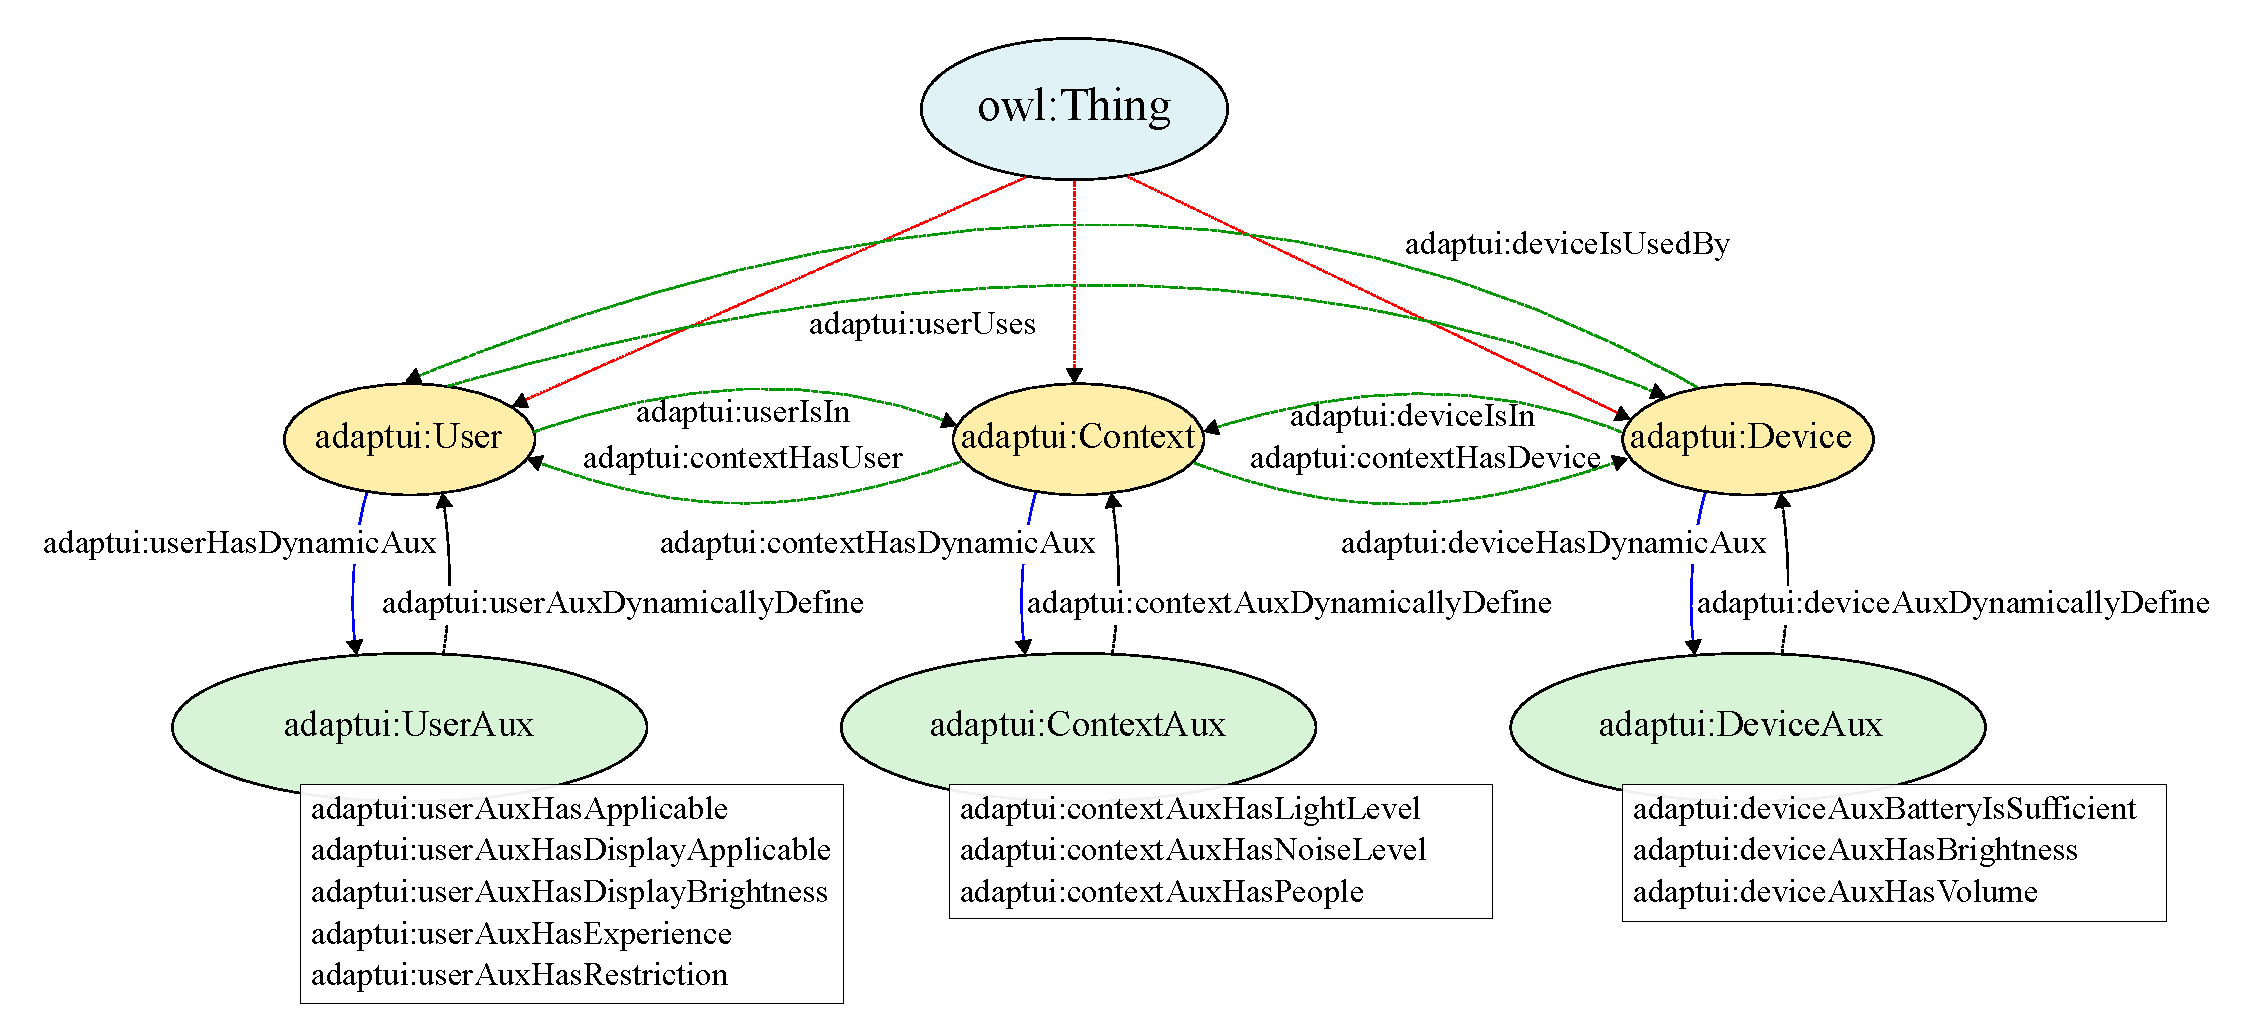
\includegraphics[width=1.0\textwidth]{../figures/PDF/auxiliary_classes.pdf}
\caption{\textit{UserAux}, \textit{ContextAux} and \textit{DeviceAux} classes
(in yellow) and their main datatype relationships.}
\label{fig:auxiliary_classes}
\end{figure}

As said before, AdaptUI allows users to manage the adaptation model through the
Capabilities Collector module. This idea, based on the work by~\citet{razmerita_ontology_based_2003},
allows users to participate during the model personalization and adaptation process. 
To this end, several classes have an \textit{isStatic} data property. This property
enables or disables the adaptation for the corresponding class depending on its
value (\textit{true} or \textit{false}). For example, the user might not want the
display brightness to be changed. A user profile where the brightness is configured
as static with the corresponding boolean value (\textit{adaptui:userdisplayBrightnessIsStatic})
means that during the adaptation process the corresponding rule (see the adaptation
rules set in Section~\ref{sec:adaptui_rules}) will evaluate this property
and finally avoid any change for the brightness parameter. The set of AdaptUIOnt
classes, object and datatype properties are shown through Figure~\ref{fig:classes},
Figure~\ref{fig:object_properties} and Figure~\ref{fig:datatype_properties}
respectively.

%CLASSES
\begin{figure}
\centering
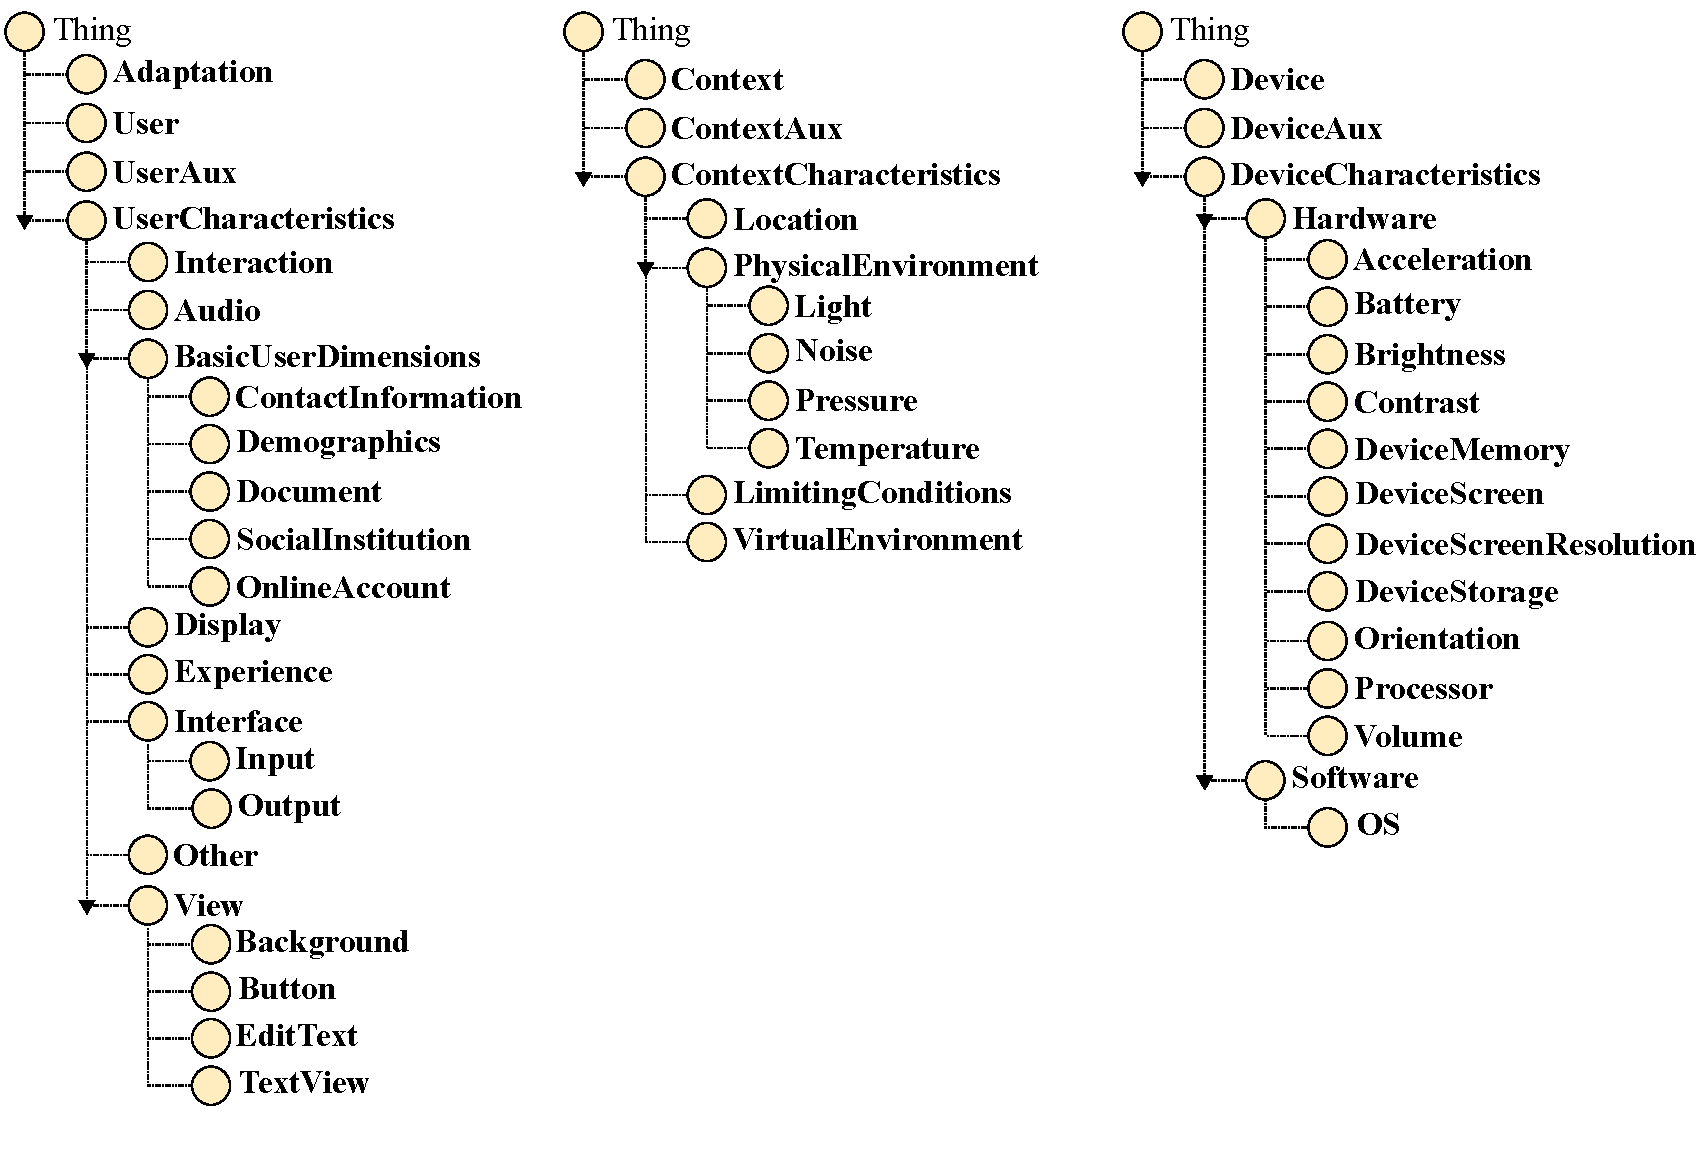
\includegraphics[width=0.95\textwidth]{../figures/PDF/classes.pdf}
\caption{\textit{User} (left), \textit{Context} (centre)
and \textit{Device} (right) classes of the AdaptUI ontology.}
\label{fig:classes}
\end{figure}

%OBJECT PROPERTIES
\begin{figure}
\centering
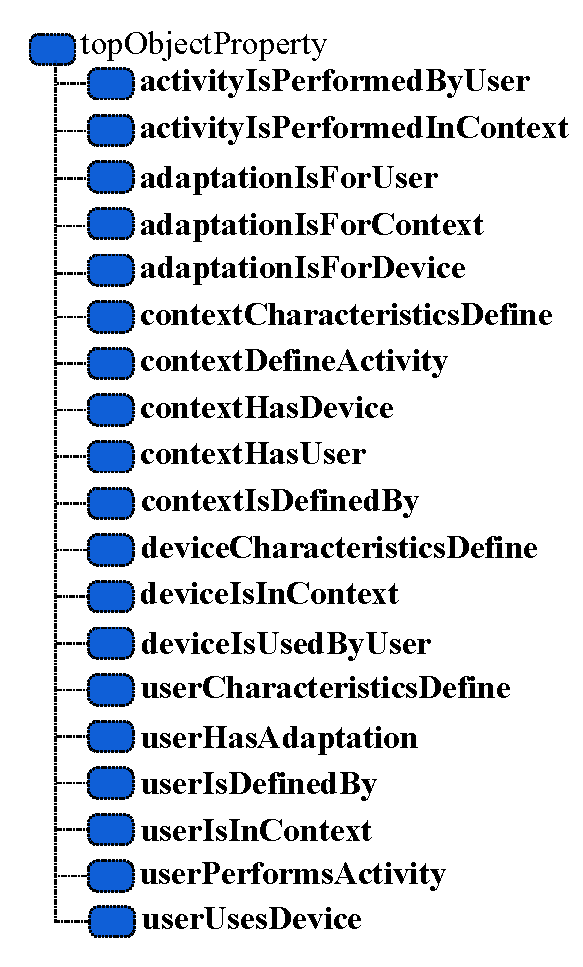
\includegraphics[width=0.33\textwidth]{../figures/PDF/object_properties.pdf}
\caption{AdaptUI object properties.}
\label{fig:object_properties}
\end{figure}

%DATATYPE PROPERTIES
\begin{figure}
\centering
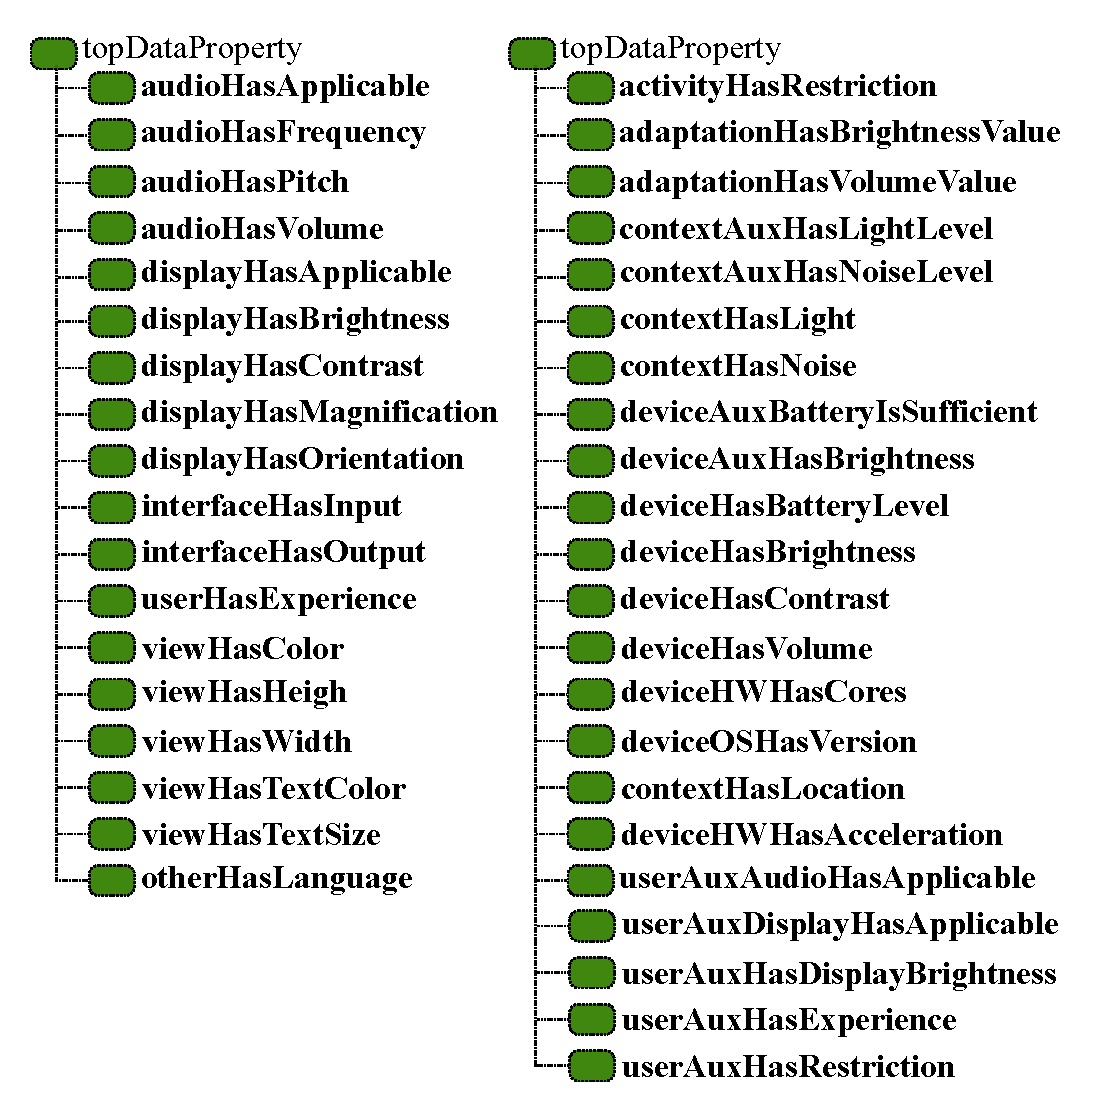
\includegraphics[width=0.65\textwidth]{../figures/PDF/datatype_properties.pdf}
\caption{AdaptUI datatype properties, not considering other ontologies. The left
group of properties are those related to
the \textit{UserCharacteristics} class.}
\label{fig:datatype_properties}
\end{figure}


\subsection{The \textit{Entities Model}}
\label{sec:entities_model}

After reviewing the literature in Chapter~\ref{cha:state_of_the_art} we found
that, for an appropriate adaptation of a user interface, there are three main
entities which must be represented in the domain: the user, the context and the
device. These concepts are semantically represented through the \textit{User},
\textit{Context} and \textit{Device} classes in the AdaptUIOnt ontology. But 
these three classes do not represent these entities alone. They are defined by 
their corresponding characteristics. These characteristics are represented through 
the \textit{UserCharacteristics}, \textit{ContextCharacteristics} and
\textit{DeviceCharacteristics} classes (see Figure~\ref{fig:user_characteristics_class}).
Together with the \textit{Adaptation} class, these seven classes form the Entities
Model, which is a conceptual group within the whole AdaptUIOnt model.
Figure~\ref{fig:entities_characteristics} shows the set of classes which form
the Entities Model.

\begin{figure}
\centering
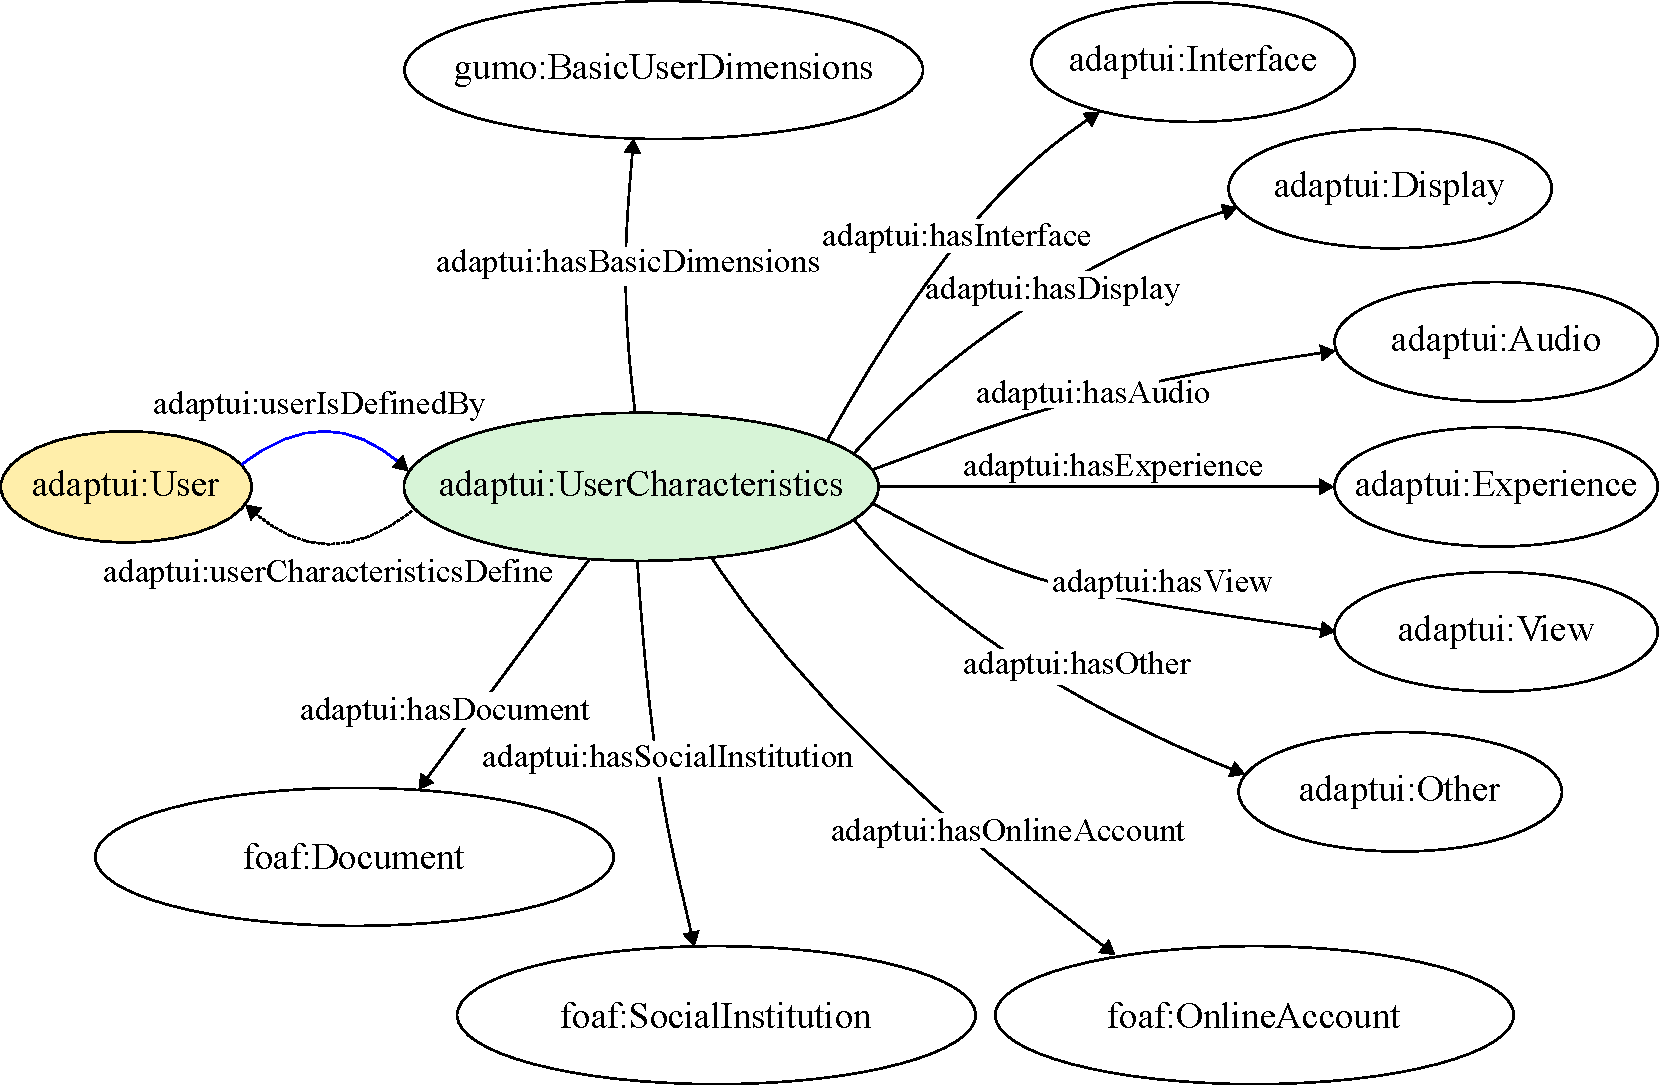
\includegraphics[width=0.85\textwidth]{../figures/PDF/user_characteristics_class.pdf}
\caption{The \textit{User} and the \textit{UserCharacteristics} classes.}
\label{fig:user_characteristics_class}
\end{figure}

Through the following sections the classes which belong to the Entities Model
are detailed. First, the \textit{UserCharacteristics} class is described in
Section~\ref{sec:user_characteristics_class}. Next, the \textit{ContextCharacteristics}
class is detailed (see Section~\ref{sec:context_characteristics_class}). Third,
a description of the \textit{DeviceCharacteristics} class is given in
Section~\ref{sec:device_characteristics_class}. Finally, the \textit{Adaptation}
class is detailed in Section~\ref{sec:adaptation_class}.


\subsubsection{The \textit{UserCharacteristics} Class}
\label{sec:user_characteristics_class}

The \textit{UserCharacteristics} class is one of the seven classes included in
the conceptual Entities Model. This class includes a series of subclasses which
build the knowledge about the user. Several user modelling ontologies are used
(i.e., \ac{foaf}~\citep{foaf} and \ac{gumo}~\citep{heckmann_gumogeneral_2005}). 
However, the strength of this class lies not on the representable knowledge 
through these classes, but in the way the knowledge about the user capabilities
(and disabilities) is represented. As explained in the introduction of this 
chapter, modelling physiological capabilities of users is troublesome and not 
practical. Several authors have tried to model user physiological characteristics~\citep{gregor_designing_2002}
\citep{razmerita_ontology_based_2003}~\citep{pereira_triple_2005}~\citep{persad_characterising_2007}
\citep{persad_cognitive_2007} and~\citep{skillen2012ontological}. Although their
systems may behave properly, there is still the issue of facing a coherent user
modelling process including user's capabilities. Not only because we lack
physiological background in the area, but also because different users may behave
in different ways even if they suffer from the same disability. 

To avoid this problem and to provide an ontology able to model user's 
capabilities, AdaptUIOnt's user's capabilities and disabilities knowledge is 
represented through the following classes:

\begin{itemize}
  \item \textit{Interface}: This category gathers input and output information
  about the user interaction preferences. Instead of modelling physiological
  capabilities regarding user's interaction abilities (e.g., sight capabilities),
  the model focuses in taking into account the user needs. For example, a user
  with a sight problem will not have to model a specific sight disability. This
  would require to consider several sight conditions and, for each one, different
  measures, ranges and classifications. Instead of that, there is the possibility
  for the user to model the Input/Output as voice and audio based interaction
  (by default the interaction is established as \textit{haptic}). This means that,
  by specifying these parameters, the system will understand that the user might
  suffer from a hearing loss condition or a sight disability.
  Table~\ref{tbl:user_characteristics_ontology} shows the interaction channels
  modelled by default in AdaptUIOnt.

  \item \textit{Audio} and \textit{Display}: These two classes model aspects
  about the use of the audio commands and volume controls, as well as different
  presentation parameters for the display, as brightness, contrast, orientation
  and magnification (see all the properties in Table~\ref{tbl:user_characteristics_ontology}).
  Thus, sight disabilities or, simply, sight problems due to context conditions
  (e.g., direct sunlight on the device screen) and hearing problems are faced by
  allowing the user to establish the default (or minimum) brightness, magnification,
  contrast, pitch, frequency and volume of the adaptation.
    
  \item \textit{Experience}: User experience with technology might be useful when
  executing adaptation rules. For examples, inexperienced users may need more
  instructions to run the profile (model) configuration process to add the
  corresponding knowledge about their capabilities.
  
  \item \textit{Other}: Several extra parameters (for example, the property
  \textit{has\_TTS}, which means that the user needs a tool which reads the text from
  the display). It also includes language and vibration related aspects.
  
  \item \textit{View}: User interfaces are composed of different views (\acs{gui} 
  elements) that are combined for representing different applications and services. 
  For each of these views (e.g., a button) the model considers several properties 
  that the user can configure (i.e., size and colours). For example, users with 
  colour blindness can change the colours of the components before any adaptation 
  to specify the set of colours they are able to distinguish, or adjust a 
  minimum size for a button so the user is able to interact with it. Thus, in 
  the future adaptations, the adaptation rules will be aware of this user 
  particular need.
  
  \item \textit{Basic User Dimensions}: Extracted from the \ac{gumo} ontology
  \citep{heckmann_gumogeneral_2005}, this class models information about the user
  contact information. See Table~\ref{tbl:used_ontologies} in order to see the
  whole set of classes included under this class.
  
  \item \textit{Document}, \textit{SocialInstitution} and \textit{OnlineAccount}:
  Extracted from \ac{foaf}~\citep{foaf}, these classes complete several personal 
  and social characteristics of the user.
\end{itemize}



\begin{center}
\footnotesize
\begin{longtable}{l l l}
  
  \label{tbl:user_characteristics_ontology} \\
  \hline 
  \textbf{Subclass} 	& \textbf{Property name} 	& \textbf{Description}							\\
  \hline
  \textit{Interface}	& \textit{interfaceHasInput}	& This property models the possible input methods for the		\\
			& 				& user with the following possibilities: \textit{gestures}, \textit{haptic},\\
			& 				& \textit{voice\_control}, \textit{sensory}, \textit{only\_haptic}, \textit{only\_voice\_control}.\\
			& \textit{interfaceHasLanguage}	& Describes to define the desired language. 				\\
			& \textit{interfaceHasOutput}	& This property models the possible output  methods for 		\\
			& 				& the user with the following possibilities: \textit{standard}  	\\
			& 				& (images, text, video and sound), \textit{only\_audio}, \textit{only\_text}.	\\
  
  \textit{Audio}	& \textit{audioHasApplicable}	& Describes if audio interaction is applicable for the user. 		\\ 
			& 				& If \textit{false}, we infer that the user might suffer from		\\
  			& 				& some hearing problems.						\\
  			& \textit{audioHasFrequency}	& Represents the preferred audio frequency. 				\\
  			& \textit{audioHasPitch}	& Describes the preferred pitch. 					\\
  			& \textit{audioHasVolume}	& Represents value which points out the desired audio 			\\
  			&				& volume.								\\
  			
  \textit{Display}	& \textit{displayHasApplicable}	& Describes the capability of the user to interact with			\\
			& 				& the display. If \textit{false} we might understand that the user 	\\
			& 				& suffers from a sight disability.		 			\\
			& \textit{displayHasBrightness}	& Represents value representing the brightness value.			\\
			& \textit{displayHasContrast}	& Describes indicating the contrast value.				\\
			& \textit{displayHasMagnification}& Represents value which represents the magnification			\\ 
			&				& degree needed for the user to properly see the display.		\\
			& \textit{displayHasOrientation}& Describes two options: \textit{landscape} or \textit{portrait}.  	\\
			& 				& This parameter indicates the preferred display 	 		\\
			&				& orientation for the user.						\\
  
  \textit{Experience}	& \textit{userHasExperience}	& A set of possible values to describe user's experience 		\\
			& 				& qith technology: \textit{standard}, \textit{advanced}, \textit{not\_applicable}.\\
  
  \textit{View}		& \textit{viewHasColor}		& Describes the colour for the view background.				\\
			& \textit{viewHasWidth}		& Represents value to determine the width of the view.			\\
			& \textit{viewHasHeight}	& Describes the height of the view.					\\
			& \textit{viewHasTextColor}	& Represents value representing the colour for the text.		\\
			& \textit{viewHasTextSize}	& Represents value representing the text size.				\\
  \hline 
\caption{UserCharacteristics data properties}
\end{longtable}
\end{center}


\subsubsection{The \textit{ContextCharacteristics} Class}
\label{sec:context_characteristics_class}

Usually, context is modelled considering that the data collected by sensors is
enough to characterize it. In AdaptUIOnt this kind of context is also modelled,
since sensor information is significantly relevant for being aware of the context
environment conditions. Thus, the information collected by sensors is represented
under the \textit{PhysicalEnvironment} and \textit{Location} classes, which are
classes from the \ac{gumo}~\citep{heckmann_gumogeneral_2005} ontology. Nevertheless,
the AdaptUIOnt ontology does not only model sensor related knowledge. There are
three extra classes which aim modelling high-level information about the
environment: \textit{LimitingConditions}, \textit{VirtualEnvironment} and
\textit{EnvironmentMetadata}. In the following lines a description of each class
is presented:

\begin{itemize}
 \item \textit{PhysicalEnvironment}: Environment information collected from
 sensors (e.g., absolute location, available resources, light and noise conditions).
 
 \item \textit{Time} and \textit{Location}: Both classes are used to characterize
 each user and device in a temporal and location context. Both entities are linked
 to these context variables through the \textit{userIsIn} and \textit{deviceIsIn}
 object properties (see Figure~\ref{fig:object_properties}).
 
 \item \textit{LimitingConditions}: Instead of modelling a set of particular
 activities we consider several context situations that might impede the interaction
 with the user. These situations are modelled as different groups regarding the
 capabilities that they might affect.
 
 \item \textit{VirtualEnvironment}: Combining the knowledge of the categories
 above, it is possible to extract high-level information. For example, sensing
 that there is a light at the office, it is possible to infer that there are
 people working. Thus, we avoid the use of other sensors to indicate this
 activity.
 
 \item \textit{EnvironmentMetadata}: Environment knowledge is associated to
 sensors. A sensor can provide information about the temperature (23 ºC). But
 this information by itself is poor in a context-aware system. Environment metadata
 can describe and enrich this knowledge, providing time and location data. For
 example, ``the current temperature at 12:00 AM in Bilbao is 13 ºC''.
\end{itemize}


Table~\ref{tbl:context_characteristics_ontology} shows the main datatype properties
of the \textit{ContextCharacteristics} class.

\begin{table}[H]
  \caption{ContextCharacteristics data properties}
 \label{tbl:context_characteristics_ontology}
\footnotesize
\centering
 \begin{tabular}{l l l}
  \hline 
  \textbf{Subclass} 	& \textbf{Property name} 	& \textbf{Description}		\\
  \hline
  \textit{Location}	& \textit{hasRelativeLocation}	& Represents relative locations.\\
			& \textit{hasAbsoluteLocation}	& Describes \textit{longitude} and \textit{latitude}.\\
  \textit{Light}	& \textit{contextHasLight}	& Describes the amount of \ac{lx}\\
			& 				& in the environment.		\\
  \textit{Noise}	& \textit{contextHasNoise}	& Represents the amount of \acp{db}\\
			& 				& in the environment.		\\
  \textit{Time}		& \textit{hasTimeValue}		& The current time.		\\
  \textit{LimitingConditions}& \textit{hasMovementRestriction}&				\\
  \hline
  
\end{tabular}
\end{table}



\subsubsection{The \textit{DeviceCharacteristics} Class}
\label{sec:device_characteristics_class}

The device model is also built over several useful classes from other ontologies.
The most important characteristic of this class consists in modelling dynamic
information about the device regarding the adaptation. For example, low battery
levels might be considered risky by the AdaptUI system, as there is the possibility
that the device turns off during the process. Device capabilities are categorized
as follows:

\begin{itemize}
 \item \textit{Software}, which encompasses different software aspects of the
 device (i.e., the \ac{os} platform). 
 
 \item \textit{Hardware}, designed to model information about the current status
 of different capabilities (i.e., available battery and memory).
\end{itemize}


Table~\ref{tbl:device_characteristics_ontology} shows the main datatype properties
of the \textit{DeviceCharacteristics} class.


\begin{table}
  \caption{DeviceCharacteristics data properties.}
 \label{tbl:device_characteristics_ontology}
\footnotesize
\centering
 \begin{tabular}{l l l}
  \hline 
  \textbf{Subclass} 	& \textbf{Property name} 	& \textbf{Description}		\\
  \hline
  \textit{Brightness}	& \textit{deviceHasBrightness}	& Describes the current		\\
			& 				& device's brightness.		\\
  \textit{Contrast}	& \textit{deviceHasContrast}	& Represents the current 	\\
  			& 				& device's contrast.		\\
  \textit{Volume}	& \textit{deviceHasVolume}	& Describes the current		\\
   			& 				& device's volume.		\\
  \textit{Processor}	& \textit{deviceHasHWCores}	& Models the number 		\\
			& 				& of the device's cores.	\\
  \textit{OS}		& \textit{deviceOSHasVersion}	& Indicates the current		\\
			& 				& \ac{os} version.		\\
  \textit{Acceleration}	& \textit{deviceHasAcceleration}& Represents the current 	\\
			& 				& X, Y, Z acceleration.		\\
  \textit{DeviceScreen,	Processor,}& \textit{hasFactoryValue}& Maximum values for 	\\
\textit{Orientation, DeviceMemory,}& 			& the elements under the  	\\
\textit{Battery, DeviceScreenResolution,} & 		& Sub-class column.  		\\
\textit{DeviceStorage} 	& 				& 				\\
  \hline

\end{tabular}
\end{table}


\subsubsection{The \textit{Adaptation} Class}
\label{sec:adaptation_class}

The last class included in the Entities Model is the \textit{Adaptation} class.
This class represents the final stage of the whole adaptation process. This means
that, after the adaptation process the results will be represented through an
individual (or instance) of this class. Therefore, the AdaptUI platform will
semantically request the corresponding adaptation for the user interface to this
class. As can be seen in Figure~\ref{fig:entities_characteristics}, the
\textit{Adaptation} class is linked to the other classes of the Entities Model
(\textit{User}, \textit{Context} and \textit{User}) through the \textit{adaptationIsDefinedBy}
object property. Thus, future semantic requests are allowed searching for a
specific user capability, context situation or device characteristics.
Table~\ref{tbl:adaptation_properties} shows the datatype properties of the
\textit{Adaptation} class.


\begin{table}
  \caption{\textit{Adaptation} class datatype properties.}
 \label{tbl:adaptation_properties}
\footnotesize
\centering
 \begin{tabular}{l l}
  \hline 
  \textbf{Datatype property} 			& \textbf{Description}				\\
  \hline
  \textit{adaptationBrightnessHasValue}		& Describes the final brightness value to be 	\\
						& configured in the device. 			\\
  \textit{adaptationVolumeHasValue}		& Represents the final volume value to be 	\\
						& configured in the device. 			\\
  \textit{adaptationButtonHasSize}		& Describes the final size value for a button. 	\\
  \textit{adaptationButtonHasBackgroundColor}	& Represents the final background colour for 	\\
						& a button.					\\
  \textit{adaptationButtonHasTextSize}		& Describes the final text size for a button.	\\
  \textit{adaptationButtonHasTextColor}		& Represents the final text colour for a button.\\
  \textit{adaptationEditTextHasSize}		& Describes the final size value for a edit text.\\
  \textit{adaptationEditTextHasBackgroundColor}	& Represents the final background colour for 	\\ 
						& a edit text.					\\
  \textit{adaptationEditTextHasTextSize}	& Describes the final text size for a edit text.\\
  \textit{adaptationEditTextHasTextColor}	& Represents the final text colour for a edit text.\\
  \textit{adaptationTextViewHasSize}		& Describes the final size value for a text view.\\
  \textit{adaptationTextViewHasBackgroundColor}	& Represents the final background colour for 	\\
						& a text view.					\\
  \textit{adaptationTextViewHasTextSize}	& Represents the final text size for a text view.\\
  \textit{adaptationTextViewHasTextColor}	& Describes the final text colour for 		\\
						& a text view.		 			\\
  \hline
  
\end{tabular}
\end{table}


% \section*{}


\subsection{Incoherence and Activities}
\label{sec:incoherence}

During the design of the AdaptUI ontology we have considered how the three
main entities (user, context and device) interact with each other. Modelling
these entities and being aware of the interactions that occur among them help
us to deduce the best adaptation for the user in each case. However, there are
several situations where the adaptation process is not so obvious. These situations
are defined by the activities that are being carried out within the environment.

\citet{persad_characterising_2007}~\citep{persad_cognitive_2007}
consider that activities need to be taken into account. They describe Human
Factors and Ergonomic theory as four components: the user, the product, the context
and the activities over time that constitutes the interaction.
\citet{hong_context_aware_2009} classify context conflicts into several categories:

\begin{itemize}
 \item Sensing conflict: Not matching results from several physical data sources.
 
 \item Service resource conflict: The lack of resources in a service offering
 process may provoke several conflicts.
 
 \item User preference conflict: Users whose profiles or preferences are different
 but having the same context situation may also result in context conflict.
\end{itemize}

During the designing process of AdaptUI, we asked ourselves if it would be enough
to consider just the user and his/her capabilities within the current context.
Thus, several hypothetical scenarios were studied:

\begin{itemize}
 \item A user suffers from a visual impairment. This disability obstructs
 the user from seeing the application content properly. Then the adaptation
 will intercede to facilitate another interaction channel for the user, e.g.,
 by voice recognition and control. The problem is that there are situations
 in which a common adaptation from the system will not be appropriate.
 For example, if the user is in a place where silence is essential (i.e., a
 library, a hospital or in an exam), an audio interaction based communication
 could not be appropriate. 
 
 \item A user who sees perfectly well interacts with the application's
 default user interface. If we avoid a situation in which the user is driving
 a visual/touch based adaptation could put the user in risk, as he/she would
 need to look at the display and use his/her hands.
 
 \item Another user is at home, and he/she does not suffer from any severe
 disability. At 01:00 pm he/she starts cooking. The application requests
 user attention for several tasks. This situation might be risky if the adaptation
 requests the user attention while he/she has, for example, oil in the pot, or
 he/she is manipulating knives.
\end{itemize}

These examples show several situations where users are involved in tasks that
contradict the current context and user capabilities. Adaptation incoherence is
defined by several environment parameters that induce the platform to perform a
certain adaptation for the current conditions. However, the result of this
adaptation, although it can be aligned with the context characteristics, can be
incoherent.

Therefore, we need something more to characterize the current situation that
involves these three entities: activities. Activities help us to understand the
current user, context and device situation. In other words, it enriches the
environment information.

Requiring the use of the hands, being at a certain location (like a library, where
people has to be in silence), or demanding the user attention are several examples
of situations which may represent some risks that we have to take into account
when we face a context modelling problem. For example, driving or cooking restricts
user capabilities momentarily. Hence, we can state that these activities impede
the user. As is difficult to model every possible activity that the user performs,
in AdaptUI we present a class (\textit{LimitingConditions}) that models abstract
groups of activities:

\begin{itemize}
 \item Activities that limit the use of the hands.
 \item Activities that limit the use of the voice.
 \item Activities that limit the user sight capability.
 \item Activities that limit the user attention.
 \item Activities that limit the user movement.
 \item Combinations of these activities.
\end{itemize}

\subsection{The \textit{Dynamic Model}}
\label{sec:dynamic_model}

The proposed solution addresses several issues of several modelling approaches
found in the literature. Following the perspective of~\citet{fischer_user_2001}
we consider that the modelled entities are not static at all. They change through
time due to their interaction. To express this concept of \textit{dynamic model}
we have implemented several auxiliary classes:

\begin{itemize}
 \item \textit{UserAux}: This class is helpful when a certain context situation
 impedes a user capability. Updated by the pre-adaptation rules this class is used
 as intermediary between the \textit{Adaptation} class and the \textit{ContextAux}
 class, where the classification of the context collected information is modelled.
 As is shown in Table~\ref{tbl:aux_classes_data_properties}, it models several user
 dynamic capabilities.
 
 \item \textit{ContextAux}: Context is considered in a different way. As context
 information comes from sensors, we have to translate the different incoming data
 to a more descriptive language. Thus, if a value of 35,000 lux is collected (as
 a brightness value of the \textit{ContextCharacteristics} class) we modify the
 contextAuxHasLightLevel data property with the \textit{direct\_sunlight} value (see
 Table~\ref{tbl:aux_classes_data_properties}). Therefore, it is possible to work
 with more meaningful data. The same occurs with the contextAuxHasNoiseLevel
 data property. Table~\ref{tbl:luminance} and Table~\ref{tbl:sounds} show the
 different classifications for light and noise levels used for AdaptUI.
 
 \item \textit{DeviceAux}: Following the same approach, this class deals with the
 dynamic capabilities of the device.
\end{itemize}

Working with sensor data opens new fronts regarding the AdaptUI platform. For
example, fuzzy reasoning would help to refine the collected information. This
is discussed in the Future Work section (see Section~\ref{sec:future_work}).


\begin{center}
\footnotesize
\begin{longtable}{l l l}
  \label{tbl:aux_classes_data_properties} \\
  \hline 
  \textbf{Class} 	& \textbf{Property name} 		& \textbf{Description}					\\
  \hline
  \textit{UserAux}	& \textit{userAuxDIsplayHasApplicable}	& Models the applicability of display adaptations for	\\
			& 					& the user. There are two different scenarios: 1) in 	\\
			& 					& the first one, the user might suffer from a 	\\
			&					& disability that makes impossible for him/her to	\\
			&					& interact with a display. In this case \textit{Display}\\
			& 					& is not applicable for this user; 2) on the contrary,	\\
			& 					& the user can specify that he/she does not want the 	\\
			& 					& display to be adapted. In any case the value of this	\\
			&					& property will determine if the rules need to consider	\\	
			& 					& \textit{Display}.					\\
			& \textit{userAuxAudioHasApplicable}	& Similar to the previous property, this one has the	\\
			& 					& same effect for audio adaptations.			\\
			& \textit{userAuxHasDisplayBrightness}	& Depending on the value of the \textit{UserCharacteristics}:\\
			& 					& \textit{userDisplayBrightnessIsStatic} property, the 	\\
			&					& corresponding rule will update this value indicating 	\\
			& 					& if the brightness should be considered for the 	\\
			&					& adaptation process.					\\
			& \textit{userAuxHasExperience}		& Represents user's experience with technology: \textit{easy},\\
			& 					& \textit{expert}, \textit{not\_possible}, \textit{standard}.\\
			& \textit{userAuxHasRestriction}	& User's activities are considered for adaptation. 	\\
			&					& Hence, a Boolean value is modelled in this property 	\\
			& 					& to indicate so.					\\
  \textit{ContextAux}	& \textit{contextAuxHasLightLevel}	& Represents several light classifications: \textit{clear\_night},				\\
			& 					& \textit{dark\_overcast}, \textit{daylight}, \textit{direct\_sunlight}, \textit{living\_room}, \\
			& 					& \textit{moonless\_clear}, \textit{moonless\_overcast}, \textit{office\_hallway}, 		\\ 
			& 					& \textit{office\_lightning}, \textit{overcast\_day}, \textit{sunrise}, \textit{twilight}.	\\
			& \textit{contextAuxHasNoiseLevel}	& Represents several noise classifications:							\\
			&					& \textit{absolute\_threshold\_of\_hearing}, \textit{breathing}, 				\\
			& 					& \textit{building\_work}, \textit{conversation}, \textit{factory},  				\\ 
			& 					& \textit{gig}, \textit{jackhammer}, \textit{leaves\_murmuring}, \textit{library},  		\\
			&					& \textit{office},  \textit{traffic}, \textit{train}, \textit{truck}, \textit{whispering}.	\\
  \textit{DeviceAux}	& \textit{deviceAuxBatteryIsSufficient}	& Based in Table~\ref{tbl:batteries}, indicates whether the \\
  			& 					& adaptation should be performed considering the 	\\
  			&					& current battery level.				\\
  			& \textit{deviceAuxHasBrightness}	& Describes the current brightness level of the device's\\
  			& 					&  screen.						\\
  \hline
\caption{Auxiliary classes' data properties.}\\
\end{longtable}
\end{center}



\begin{table}
  \caption{Luminance provided under various conditions~\citep{luminance}.}
 \label{tbl:luminance}
\footnotesize
\centering
 \begin{tabular}{l l l}
  \hline 
  \textbf{Brightness} & \textbf{Surfaces illuminated by}		& \textbf{Ontology value}	\\
  \textbf{(measured) in \ac{lx}}&					&				\\
  \hline
  0.0001		& Moonless, overcast night sky (starlight)	& \textit{moonless\_overcast}	\\
  0.002 		& Moonless clear night sky with air-glow	& \textit{moonless\_clear}	\\
  0.27-1.0		& Full moon on a clear night			& \textit{full\_moon}		\\
  1.0-3.4		& Dark limit of civil twilight under a clear sky& \textit{twilight}		\\
  3.4-50		& Family living room lights			& \textit{living\_room}		\\
  50-80 		& Office building hallway/toilet lighting	& \textit{office\_hallway}	\\
  80-100		& Very dark overcast day			& \textit{dark\_overcast}	\\
  320-500		& Office lighting				& \textit{office\_lightning}	\\
  500-1,000		& Overcast day; typical TV studio lighting	& \textit{overcast}		\\
  1,000-25,000		& Full daylight (not direct sun)		& \textit{daylight}		\\
  25,000-130,000	& Direct sunlight (latter figure is 		& \textit{direct\_sunlight}	\\
			& above atmosphere)				& 				\\
  \hline

\end{tabular}
\end{table}


In order to describe the whole detailed model and how the main classes are related
to each other, Figure \ref{fig:flow_diagram} shows how the knowledge flows through
the AdaptUI platform. First, the three main classes of the \textit{Entities Model}
are populated with the information about the user, the context and the device.
Then, the pre-adaptation rules are triggered and updates classifies and updates
the collected knowledge into intermediate knowledge. This knowledge is represented
in the \textit{UserCharacteristics}, \textit{ContextCharacteristics} and
\textit{DeviceCharacteristics} classes. Finally, the \textit{Adaptation} class
requests the processed knowledge and through the adaptation rules the final
adaptation is sent to the user. Additionally, within the user model the interaction
model collects information about the interaction, updating the \textit{UserAux}
class if needed. This brings the execution of the rules again, which means that
a new result is generated.


\begin{table}[H]
  \caption{Most common sound intensity levels modelled by default in AdaptUI.}
 \label{tbl:sounds}
\footnotesize
\centering
 \begin{tabular}{l r}
  \hline 
  \textbf{Ontology value}	& \textbf{\ac{db}}\\
  \hline
  Absolute threshold of hearing	& 0	\\
  Breathing			& 10 	\\
  Leaves murmuring		& 20	\\
  Library			& 40	\\
  Office			& 50	\\
  Conversation			& 60	\\
  Traffic			& 70	\\
  Factory			& 80	\\
  Truck				& 90	\\
  Train				& 100	\\
  Construction			& 110	\\
  Rock gig			& 120	\\
  Jackhammer			& 130	\\
  \hline

\end{tabular}
\end{table}


\begin{table}[H]
  \caption{Battery percentage and ontology values for AdaptUI.}
 \label{tbl:batteries}
\footnotesize
\centering
 \begin{tabular}{c l}
  \hline 
  \textbf{Battery (\%)} 	& \textbf{Ontology value}	\\
  \hline  
  $x\leq15$			& Not sufficient		\\
  $15<x\leq50$			& Sufficient			\\
  $50<x\leq100$			& Optimal			\\
  \hline

\end{tabular}
\end{table}



\subsection{Conclusions}
\label{sec:model_conclusions}

During the previous sections the AdaptUIOnt ontology, which forms part of the two
main bases of the AdaptUI platform, has been described. The most significant
characteristic of the ontology is that allows the representation of the knowledge
about what we consider the three main entities in a user interface adaptation
domain: the user, the context, and the device. 

The first trouble when designing the ontology appeared when the user capabilities
modelling was needed. As we lack the required physiological knowledge in this area,
we believe that using physiological information of the user capabilities would
not be practical. Thus, an abstraction of the conceptualization of the model was
performed. Instead of consider the physiological factors that allow a user to
perform several interactions, the AdaptUIOnt model centres its focus in the needs
of the user to carry out these interactions. This is significant, as it allows
us to avoid these capabilities explicitly. Besides, the presented ontologies
uses several extendedly used ontologies to enrich the information about the three
entities. Table~\ref{tbl:used_ontologies} details the most important classes
imported in AdaptUIOnt.

The ontology has been conceptually divided into two different parts. The first
one gathers the main classes, those which directly represent knowledge about
the main entities. In this case, this part of the ontology has been called
Entities Model, and its composed by the \textit{User}, \textit{Context},
\textit{Device}, \textit{UserCharacteristics}, \textit{ContextCharacteristics},
\textit{DeviceCharacteristics} and \textit{Adaptation}. Each main entity is
defined by a class which models its characteristics. Thus, the \textit{User}
class is directly related to the \textit{UserCharacteristics} class through a
\textit{isDefinedBy} object property. The same procedure is followed by the other
two main entities. The \textit{Adaptation} class, however, just represents the
final stage of the whole adaptation process. Therefore, after the corresponding
reasoning (detailed in the following sections) the AdaptUI platform will
semantically requests the adaptation information represented by it.

\section{The AdaptUI Rules Set}
\label{sec:adaptui_rules}

As said in the introduction of this chapter, the developed adaptation platform is 
supported by two bases. The first one, the AdaptUIOnt ontology, described in the 
previous sections. The second one, a set of rules that uses the knowledge represented
by the ontology and triggers several actions aiming the user interface adaptation. 
In this dissertation the adaptation process is understood as a three step procedure: 

\begin{itemize}
 \item First, the knowledge of the main entities needs to be collected. Once it
 is gathered, a normalization process is performed. This process classifies the 
 collected information so it can be easily read. For example, a noise sensor
 might sense a 100~\acp{db} sound. Initially, the platform might not understand
 this value. Thus, using several ranges explained during this chapter (see 
 Table~\ref{tbl:luminance}, Table~\ref{tbl:sounds} and Table~\ref{tbl:batteries})
 a high level classification is carried out.
 
 \item Secondly, and taking into account the transformed knowledge in the previous
 step, several actions are performed to adapt the user interface to the current 
 situation (represented through the ontology in the previous stage).
 
 \item Finally, a refinement of the adapted user interface is available to improve
 the final results.
\end{itemize}

This conceptual division of the adaptation process in the adaptation platform 
results in a three set of different rules, which are detailed below.


\subsection{The Pre-adaptation Rules}
\label{sec:preadaptation_rules}

This group of rules are designed to check those values which come from each entity 
of the Entities Model in order to translate them to the auxiliary models. For 
example, a 35,000 \ac{lx} context brightness indicates the amount of \ac{lx} of the 
current environment. This value is then classified to a more verbose subgroup 
(in this case, \textit{direct\_sunlight}); a 10 device battery value represents 
the percentage of the remaining battery. This is translated as a 
\textit{non\_sufficient} battery level in the auxiliary device class. Thus, the
corresponding adaptation rule checks these new parameters and decides whether the
adaptation should follow one path or the other. In this dissertation we consider
that 10\% of the total battery levels for a device might not be enough to run an
adaptation process. Of course this is not accurate. The user might be able to
use a nearby power adaptor. Besides, 10\% battery level might not be enough if
the user aims to browse the web, make a video call, and so forth, but it might be
sufficient carrying out one adaptation. This means that these values are established
by the developer regarding the just the adaptation, but they directly depend on
the user context. This set of rules directly affects the \textit{UserAux},
\textit{ContextAux} and \textit{DeviceAux} classes, being the main reason for
these classes to belong to the Dynamic Model introduced in Section~\ref{sec:dynamic_model}.

Table~\ref{tbl:pre_adaptation_rules} describe the default pre-adaptation rules
included in AdaptUIOnt.

\begin{table}
  \caption{The AdaptUIOnt pre-adaptation rules.}
 \label{tbl:pre_adaptation_rules}
\footnotesize
\centering
 \begin{tabular}{l l l}
  \hline 
  \textbf{Pre-adaptation rule} 			& \textbf{Involved ontologies} 	& \textbf{Description} 	\\
						& \textbf{and classes} 		& 			\\
  \hline
  \textit{checkBatteryLevelIsSufficient}& \textit{soupa:Battery}	& Considering Table~\ref{tbl:batteries} this rule\\
					& \textit{adaptui:Device}	& evaluates if the current battery 		\\
					& \textit{adaptui:DeviceAux}	& level is enough to perform any 		\\
					&				& adaptation. 					\\
  \hline
  
  \textit{checkLightLevelDarkOvercast}	& \textit{adaptui:Context}	& These rules evaluate the context   		\\
  \textit{checkLightLevelTwilight}	& \textit{adaptui:ContextAux}	& light input through sensors by  		\\
  \textit{checkLightLevelSunrise}	& \textit{gumo:Light}		& using the classification shown in 		\\
  \textit{checkLightLevelOvercast}	& 				& Table~\ref{tbl:luminance}. The result of this \\
  \textit{checkLightLevelOfficeLightning}&				& evaluation would be a verbose  		\\
  \textit{checkLightLevelOfficeHallway}	&				& concept (e.g., \textit{sunrise}) which is   	\\
  \textit{checkLightLevelMoonlessClear}	&				& stored in the ontology using the  		\\
  \textit{checkLightLevelDayLight}	& 				& \textit{contextAuxHasLightLevel} datatype	\\
  \textit{checkLightLevelDirectSunlight}& 				&  property.					\\
  \textit{checkLightLevelFullMoon}	& 				& 						\\
  \textit{checkLightLevelLivingRoom}	& 				& 						\\
  \hline
  
  \textit{checkNoiseLevelBreathing}	& \textit{adaptui:Context}	& These rules evaluate the context 	 	\\
  \textit{checkNoiseLevelTruck}		& \textit{adaptui:ContextAux}	& noise input through sensors by  		\\
  \textit{checkNoiseLevelTrain}		& \textit{gumo:Noise}		& using the classification  shown in 		\\
  \textit{checkNoiseLevelTraffic}	& 				& Table~\ref{tbl:sounds}. The result of this 	\\
  \textit{checkNoiseLevelOffice}	&				& evaluation would be a verbose 		\\
  \textit{checkNoiseLevelLibrary}	&				& concept (e.g., \textit{sunrise}) which is  	\\
  \textit{checkNoiseLevelLeavesMurmuring}&				& stored in the ontology using the 		\\
  \textit{checkNoiseLevelBreathing}	&				& \textit{contextAuxHasNoiseLevel} datatype	\\
  \textit{checkNoiseLevelBuildingWork}	&				& property.					\\
  \textit{checkNoiseLevelConversation}	&				& 						\\
  \textit{checkNoiseLevelFactory}	&				& 						\\
  \textit{checkNoiseLevelGig}		&				& 						\\
  \textit{checkNoiseLevelJackhammer}	&				& 						\\
  \hline
  
  \textit{checkUserHasAttentionRestriction}& \textit{adaptui:Activity}	& If the current activity impedes the 		\\
  \textit{checkUserHasNoRestriction}	& \textit{adaptui:UserAux}	& user, these rules would store the 		\\
  \textit{checkUserHasSightRestriction}	&				& corresponding boolean value in the 		\\
  \textit{checkUserHasMovementRestriction}&				& \textit{userAuxHasRestriction} datatype 	\\
  \textit{checkUserHasHandsRestriction}	&				& property.					\\
  \textit{checkUserHasHearingRestriction}&				& 						\\
  \hline
\end{tabular}
\end{table}

Equation~\ref{ec:pre_adaptation_rule} shows an example of the 
\textit{checkNoiseLevelTraffic} pre-adaptation rule.

\footnotesize
\begin{equation} \label{ec:pre_adaptation_rule}
  \begin{align*} 
  Context(?context) \& Noise(?noise) \& ContextAux(?caux) \& \\
  contextHasNoise(?noise, ?value) \& lessThanOrEqual(?value, 70) \& \\
  greaterThan(?value, 60) \\
  \Rightarrow \\
  contextAuxHasNoiseLevel(?caux, "traffic")
  \end{align*}
\end{equation}
\normalsize


\subsection{The Adaptation Rules}
Depending on the checked rules and the auxiliary classes’ status, different 
rules are triggered. These rules result in different values for the \textit{Adaptation} 
class, which is the class queried in the device platform for bringing the final 
adaptation to the device. Table~\ref{tbl:adaptation_rules} details the default
adaptation rules in the AdaptUIOnt ontology.

\begin{table}
  \caption{The AdaptUIOnt adaptation rules.}
 \label{tbl:adaptation_rules}
\footnotesize
\centering
 \begin{tabular}{l l l}
  \hline 
  \textbf{Adaptation rule} 	& \textbf{Involved ontologies} 	& \textbf{Description} 		\\
				& \textbf{and classes} 		& 				\\
  \hline
  \textit{adaptBrightness}	& \textit{adaptui:Adaptation}	& These rules consider the  	\\
  and				& \textit{adaptui:DeviceAux}	& values stored in the 		\\
  \textit{adaptVolume}		& \textit{adaptui:UserAux}	& \textit{UserAux} class to adapt the \\
				& \textit{adaptui:Brightness}	& brightness and volume 	\\
				& \textit{adaptui:Volume}	& accordingly. 			\\
				& \textit{adaptui:Display}	& 				\\
  \hline 
  \textit{adaptButtonSize}	& \textit{adaptui:Adaptation}	& These rules take into account	\\
				& \textit{adaptui:DeviceAux}	& the current button configu-	\\
				& \textit{adaptui:UserAux}	& ration and the sensed context	\\
  \textit{adaptButtonColor}	& \textit{adaptui:Button}	& disabilities.			\\
  \textit{adaptButtonBackgroundColor}&				& 				\\
  \textit{adaptButtonTextColor}	& 				& 				\\

  \hline
  \textit{adaptEditTextSize}	& \textit{adaptui:Adaptation}	& These rules take into account	\\
				& \textit{adaptui:DeviceAux}	& the current edit text configu-\\
				& \textit{adaptui:UserAux}	& ration and the sensed	context	\\
  \textit{adaptEditTextBackgroundColor}	& \textit{adaptui:EditText}& disabilities.		\\
  \textit{adaptEditTextTextSize}& 				& 				\\
  \textit{adaptEditTextTextColor}&				& 				\\

  \hline 
  \textit{adaptTextViewtSize}	& \textit{adaptui:Adaptation}	& These rules take into account	\\
				& \textit{adaptui:DeviceAux}	& the current text view configu-\\
				& \textit{adaptui:UserAux}	& ration and the sensed	context	\\
  \textit{adaptTextViewtBackgroundColor}& \textit{adaptui:TextView}& disabilities.		\\
  \textit{adaptTextViewtTextSize}&				& 				\\
  \textit{adaptTextViewtTextColor}&				& 				\\
  \hline 
\end{tabular}
\end{table}

Equation~\ref{ec:adaptation_rule} shows an example of the \textit{adaptVolume} 
adaptation rule.

\footnotesize
\begin{equation} \label{ec:adaptation_rule}
  \begin{align*} 
  Adaptation(?adaptation) \& DeviceAux(?device) \& ContextAux(?context) \& \\
  deviceAuxBatteryIsSufficient(?device, ?battery) \& equal(?battery, true) \& \\
  contextAuxHasNoise(?context, ?noise) \& equal(?noise, ``traffic'')\\ 
  \Rightarrow \\
  adaptationVolumeHasValue(?adaptation, 7)\\
  \end{align*}
\end{equation}
\normalsize


\subsection{The Usability Rules}
In order to check the usability satisfaction of the user with the provided
adapted user interface, a usability rules set is provided. By checking several
usability metrics (detailed in Section~\ref{sec:usability_metrics}) these rules
determine if the interaction with the adapted user interface might be considered
enough. Table~\ref{tbl:usability_rules} introduced the usability rules included
in AdaptUIOnt.

\begin{table}
  \caption{The AdaptUIOnt usability rules. The metrics mentioned in this table
  are detailed in Table~\ref{tbl:effectiveness_metrics} and Table~\ref{tbl:productivity_metrics}.}
 \label{tbl:usability_rules}
\footnotesize
\centering
 \begin{tabular}{l l l}
  \hline 
  \textbf{Usability rule} 	& \textbf{Involved ontologies} 	& \textbf{Description} 		\\
				& \textbf{and classes} 		& 				\\
  \hline
  \textit{checkTaskEffectiveness}&\textit{adaptui:UserAux}	& It measures the proportion of \\
				& \textit{adaptui:Effectiveness}& goals of the task achieved	\\
				& \textit{adaptui:Polisher}	& correctly. 			\\
  \textit{checkTaskCompletion}	& 				& It measures the proportion of	\\
				& 				& the task that is completed.	\\
  \textit{checkErrorFrequency}	& 				& It measures the frequency of 	\\
				& 				& errors.			\\
  \hline
  \textit{checkTaskTime}	& \textit{adaptui:UserAux}	& It measures the required time	\\
				& \textit{adaptui:Productivity}	& to complete the current task.	\\
  \textit{checkTaskEfficiency}	& \textit{adaptui:Polisher}	& It measures the efficiency of	\\
				& 				& the user.			\\
  \textit{checkEconomicProductivity} &				& It measures the cost-effectiveness\\
				&				& of the user.			\\
  \textit{checkProductiveProportion} & 				& It measures the proportion of \\
				& 				& the time the user is performing\\
				&				& productive actions.		\\
  \textit{checkRelativeUserEfficiency}& 			& It compares the efficiency of the\\
				&				& user compared to an expert.	\\
  \hline
\end{tabular}
\end{table}

Equation~\ref{ec:usability_rule} shows an example of the \textit{checkRelativeEfficiency} 
adaptation rule.

\footnotesize
\begin{equation} \label{ec:usability_rule}
  \begin{align*} 
  UserAux(?user) \& Productivity(?productivity) \& Polisher(?polisher) \&\\ 
  userAuxHasProductivityMetrics(?user, ?productivity) \& \\
  hasRelativeEfficiency(?productivity, ?efficiency) \& \\
  lessThanOrEqual(?efficiency, 0.5) \& \\
  \Rightarrow \\
  launchPolisherRules(?polisher, true)
  \end{align*}
\end{equation}
\normalsize

\subsection{The Post-adaptation Rules}
Once the user interface is adapted, a concrete architecture module (see 
Section~\ref{sec:adaptation_polisher}) monitors the user activity. Hence, through
a series of usability metrics the adaptation is considered satisfactory by
the adaptation platform. If it detects that the usability level is inadequate,
these rules are triggered, changing the user model.

\begin{table}
  \caption{The AdaptUIOnt post-adaptation rules. For edit texts and text views
  the same rules that are applied for the buttons are provided.}
 \label{tbl:post_adaptation_rules}
\footnotesize
\centering
 \begin{tabular}{l l l}
  \hline 
  \textbf{Adaptation rule} 	& \textbf{Involved ontologies} 	& \textbf{Description} 		\\
				& \textbf{and classes} 		& 				\\
  \hline
  \textit{incrementBrightness}	& \textit{adaptui:UserAux}	& It increments the brightness of\\
				& \textit{adaptui:Polisher}	& the device in 1F.		\\
  \textit{decrementBrightness}	& \textit{adaptui:Adaptation}	& It decrements the brightness of\\
				& 				& the device in 1F.		\\
  \textit{incrementVolume}	& 				& It increments the volume of	\\
				& 				& the device in 1 unit.	\\
  \textit{decrementVolume}	& 				& It decrements the volume of	\\
				& 				& the device in 1 unit.	\\
  \hline
  \textit{incrementButtonSize}	& \textit{adaptui:UserAux}	& It increments the size of the \\
				& \textit{adaptui:Polisher}	& button adding 10 dpis. 	\\
  \textit{decrementButtonSize}	& \textit{adaptui:Adaptation}	& It decrements the size of the \\
				& 				& button in 10 dpis.		\\
  \textit{darkenButtonBackgroundColor}&				& It darkens the colour.	\\
  \textit{lightenButtonBackgroundColor}&			& It lightens the colour.	\\
  \textit{darkenButtonTextColor}&				& It darkens the text colour.	\\
  \textit{lightenButtonTextColor}&				& It lightens the text colour.	\\
  \hline
\end{tabular}
\end{table}

Equation~\ref{ec:post_adaptation_rule} shows an example of the \textit{incrementButtonSize} 
post-adaptation rule.

\footnotesize
\begin{equation} \label{ec:post_adaptation_rule}
  \begin{align*} 
  Polisher(?polisher) \& launchPolisherRules(?polisher, true) \&\\
  UserAux(?user) \& userAuxHasEffectivenessMetrics(?user, ?effectiveness) \& \\
  effectivenessMetricHasErrorFrequency(?effectiveness, ?freq?) \&\\
  greaterThan(?freq, 0.5) \& Adaptation(?adaptation) \&\\
  adaptationHasButtonSize(?adaptation, ?size)
  \Rightarrow \\
  adaptationButtonHasSize(?adaptation, ?size + 10)
  \end{align*}
\end{equation}
\normalsize



The given set of rules by the adaptation platform have been included as they are
understood as vital for a precise adaptation. Nevertheless, and as it will be
explained in Chapter~\ref{cha:architecture}, these rules are not final. This
means that they are modifiable. To this end, a series of tools for developers
that allow them to change the knowledge managed by the platform are provided.


\subsection{Conclusions}
\label{sec:rules_conclusions}

In this second part of the chapter the second main basis of the adaptation platform
has been presented: the set of rules. Divided into three different groups
(considering that the adaptation process is understood as a three step procedure)
these rules aim to finally generate a user interface adaptation under the following
steps:

\begin{itemize}
  \item Firstly, a classification and normalization of the collected knowledge of
  the main entities is needed. This might be low level knowledge. Thus, a higher
  level information is obtained during this process. To reach this goal, the
  pre-adaptation rules set is needed. These rules affect the \textit{UserAux},
  \textit{ContextAux} and \textit{DeviceAux} classes.
  
  \item Next, once the knowledge has been normalized, the adaptation rules set
  are triggered, generating the corresponding changes in the \textit{Adaptation}
  class in the AdaptUIOnt ontology.
  
  \item Finally, as the adaptation might be improvable, several rules are executed
  regarding a refinement of the last adapted user interface. This is detailed
  in Section~\ref{sec:adaptation_polisher}.
\end{itemize}
\section{AdaptUIOnt Conclusions}
\label{sec:adaptui_conclusions}

Inspired by the existing literature approaches for user, context and device
modelling in this chapter a model supported by two main bases has been described.
On the one hand, we have presented AdaptUIOnt, an ontology which deals with the
main problems analysed in Chapter~\ref{cha:state_of_the_art}. On the other hand,
a set of adaptation rules (divided into three groups: pre-adaptation, adaptation
and post-adaptation rules) have been also introduced. These two bases are
illustrated through Figure~\ref{fig:flow_diagram_2}.

The decision of using ontologies is based on the extracted conclusions from the
analysis of the literature. Specially, the analysis by~\citet{strang_context_2004}
is significantly remarked in this dissertation. In this work the authors compare
different context modelling techniques to finally conclude that ontologies
represent the most promising asset with respect to the other analysed techniques
(i.e., key-value models, markup scheme models, graphical models, object oriented
models and logic based models). As the authors state, ontologies are strong
regarding distributed composition, partial validation, content validation
and facing incompleteness and the quality of the information.

Besides, after studying the benefits extracted by~\citet{strang_context_2004}
conclusions and several significant works in the literature (see
Chapter~\ref{cha:state_of_the_art}) we found several more benefits regarding the
AdaptUIOnt model:

\begin{itemize}
  \item It makes the solution more extendible. Knowledge is easily represented
  through semantic models and the models themselves are also easily reusable.
  A context model built by others can be not only use, but for example, extended
  with ambiguity and incompleteness support. In fact, the AdaptUIOnt has been
  built over several contrasted models found in the literature (see
  Section~\ref{sec:adaptui_model}). These models are highly spread and tested
  and due to the nature of ontologies allow us to extend them with our designs.
  
  \item Reasoning is allowed over the knowledge represented in the ontology.
  Ontologies represent knowledge, and one of the benefits of using domain
  concepts is the ability to learn, classify and infer new knowledge from the
  existing one. In AdaptUI there is an architecture module which deals with
  reasoning using the knowledge stored in the AdaptUIOnt ontology (see
  Section~\ref{sec:pellet4android}).
\end{itemize}


\begin{figure}
\centering
\includegraphics[width=0.75\textwidth]{../figures/PDF/flow_diagram.pdf}
\caption{Knowledge flow through the AdaptUI adaptation process. The circles
represent several main concepts presented in the AdaptUIOnt ontology. The arrows
represent the set of rules that affect the related concepts in the circles.}
\label{fig:flow_diagram_2}
\end{figure}

However, the decision of using ontologies as a modelling technique did not only
bring benefits. The first drawback, and probably the most significant when dealing
with semantics in mobile devices, is the lack of efficiency. Examining several
approaches along the literature we encountered that, usually, the reasoning tasks
are delegated to an external infrastructure. Until the \textit{smartphones boom} (see
Figure~\ref{fig:smartphones_boom}) it was quite difficult to find mobile devices
with the appropriate hardware specifications for managing heavy processes. Thus,
the analysed literature approaches usually delegate this processing tasks to
external services (when talking about \acs{ui} adaptation in mobile devices). Then,
these services send back the corresponding results after performing the
corresponding actions. 

This drawback is significant, since AdaptUI aims to not only provide an ontology
model for the adaptation process, but also a series of tools to allow developers
to adapt the ontology and the knowledge represented through it (see 
Section~\ref{sec:knowledge_api}).


\begin{figure}
\centering
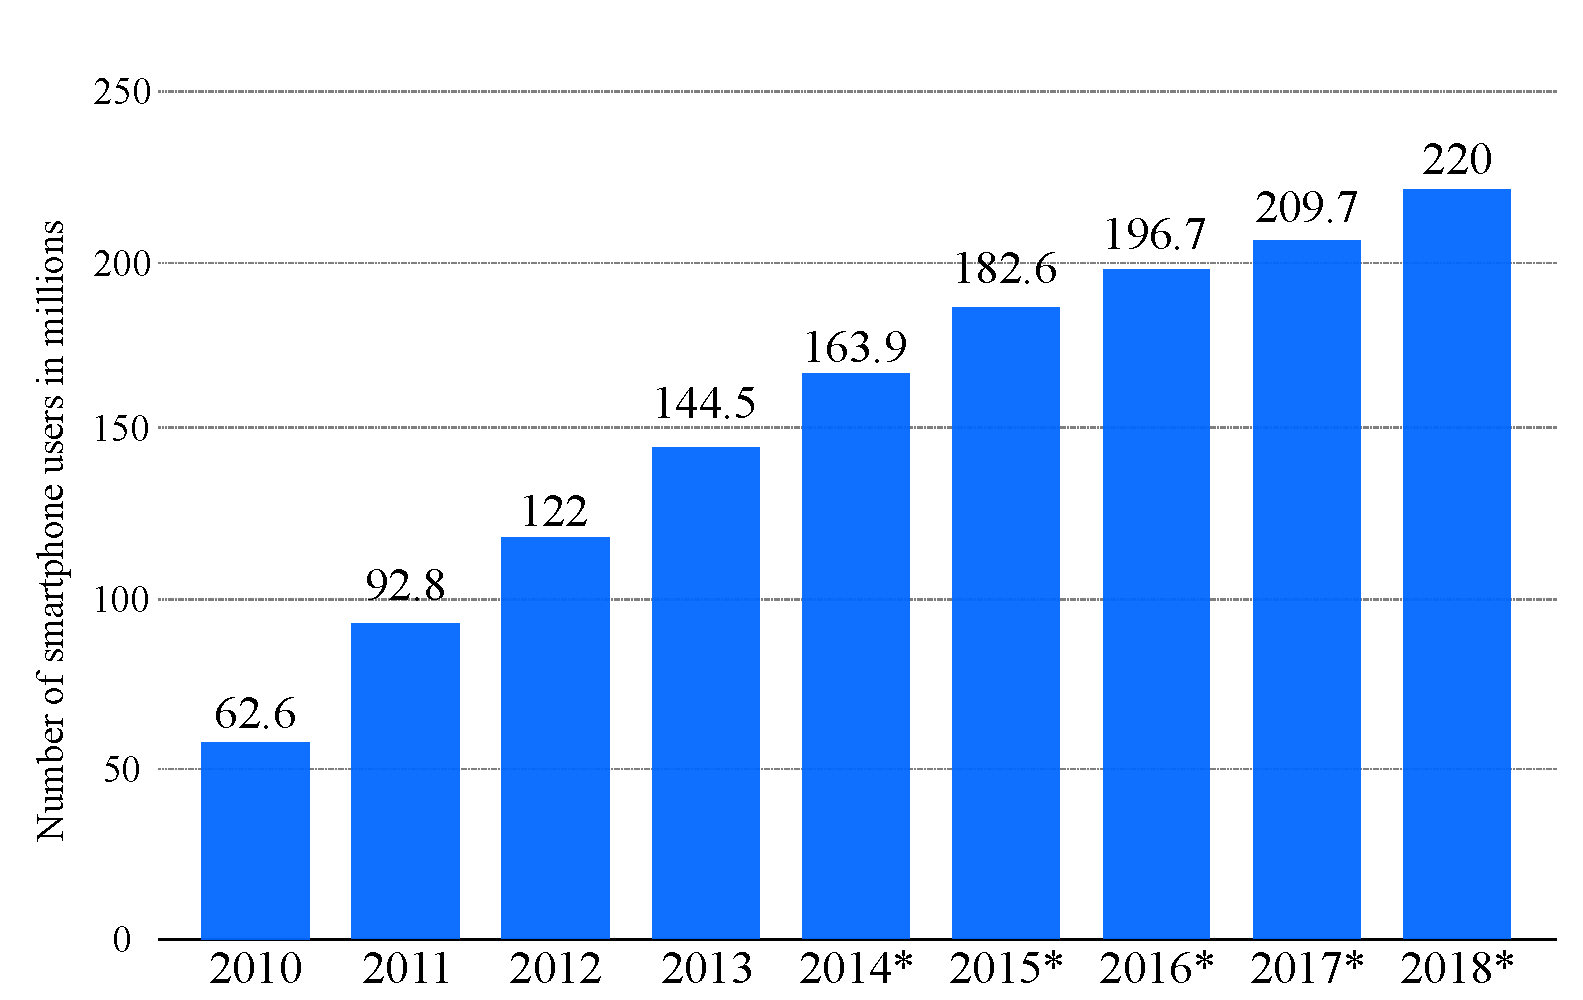
\includegraphics[width=0.85\textwidth]{../figures/PDF/smartphones_boom.pdf}
\caption{Number of smartphone users in the \ac{us} from 2010 to 2018 (in
millions)~\citep{smartphones_boom}. This forecast shows the anticipated number
of smartphone users in the \ac{us} from 2014 to 2018, based on figures from 2010 
to 2013. The source estimates that there will be more than 196 million smartphone
users in the \ac{us} by the year 2016.}
\label{fig:smartphones_boom}
\end{figure}

Another problem deals with the granularity of the model. A generic model might
not be useful for specific scenarios in the same domain, as it would lack specific
parameters. On the other hand, if it is too specific they may not apply well to
other domains. The AdaptUIOnt model tries to address this second aspect by being
abstract regarding the user disabilities. 

Regarding the presented set of rules, it is significant how they represent the
three step adaptation understood by AdaptUI. This is translated into a three
subset of rules which aim to modify and generate new knowledge through a reasoning
process. These subsets, called pre-adaptation, adaptation and post-adaptation rules,
are characterized not only for gathering several rules, but also for being modifiable
by developers through a series of tools provided by the AdaptUI platform. These
tools and their characteristics are detailed in Chapter~\ref{cha:architecture}.